\documentclass{article}

\usepackage[english]{babel}

% Set page size and margins
% Replace `letterpaper' with `a4paper' for UK/EU standard size
\usepackage[letterpaper,top=2cm,bottom=2cm,left=2cm,right=2cm,marginparwidth=1.75cm]{geometry}

% Useful packages
\usepackage{amsmath}
\setcounter{MaxMatrixCols}{15}
\usepackage{graphicx}
\usepackage[colorlinks=true, allcolors=blue]{hyperref}
\usepackage{subcaption}
\usepackage{multicol}
\usepackage{fancyhdr}
\usepackage{caption}
\usepackage{braket}
\usepackage{mathtools}
\usepackage{tikz}
\usepackage{float}
\title{Normalization and Time Alignment of TPPT}

\begin{document}
\maketitle

\tableofcontents
\newpage
\section{Introduction}
For performance of the TPPT scanner, we perform normalization and time alignment calibration. The methodology and results are described in this writeup.

\subsection{Data Acquisition and Preprocessing Cuts}
We acquire listmode data for these studies. The data is preprocessed with the following cuts to isolate true coincidences and reject obvious randoms or otherwise unphysical events. A summary is given:
\begin{enumerate}
    \item Photopeak window acceptance cut - all events involving a channel are collected and histogrammed for energy, the photopeak is fit with a gaussian and the window is defined around $2.5\sigma$ of the photopeak, events inside this window are accepted. As of 08/2026, the energy resolution of the scanner is roughly $8.2\%$. This is done for all channels.
    \item Geometric cuts - LORs are rejected if they fall outside an acceptable radius from the expected position of the source. To do this, a run is tracked as 180 discrete positions, with a corresponding time window, events within this time are accepted if they intersect within 20mm of the expected source position. This rejects LORs that clearly do not intersect the source, and is expected to correct for some randoms or otherwise unphysical events.
    \item Duplicate event cuts - if two or more events are recorded to have occured at the exact same time and in the same channel on either side, this indicates an incorrect assignment of a single event to a coincidence, and only the first event is accepted. This cut is also expected to correct for some events that would otherwise appear as randoms or otherwise unphysical events.
\end{enumerate}

We may assume that the line source is thin enough to exhibit negligible scatter, any obvious scatter events are rejected by the geometric cuts. After these cuts, the data is treated as containing only true coincidences. Additional study is needed to quantify agreement, some analysis is shown in Appendix B.

\subsection{Simulation}
We can also do simulation for certain validations and for acquiring geometric data that would otherwise be difficult to acquire with TPPT. I use Andrey's TPPTsim/TPPTbuilder/TPPTcoinc \cite{morozov_github} framework with Geant4 \cite{geant4} to simualate the generation of back to back gammas, scintillation and detection, and coincidence grouping. The following configuration is used:
\begin{itemize}
    \item No phantom, to minimize scattering for ideal study.
    \item LYSO crystal detector geometry only, again for ideal study.
    \item 1e9 back to back 511keV gammas generated uniformly in a cylinder or cylindrical shell centered at isocenter, in random direction, each use case is described later when needed. No acollinearity.
    \item Energy window: $(0.85, 1.15)\times511\text{keV}$ to roughly match our 2.5$\sigma$ photopeak window at approximately $8.2\%$ energy resolution used in our photopeak cuts on real data.
\end{itemize}
\begin{figure}[h]
    \centering
    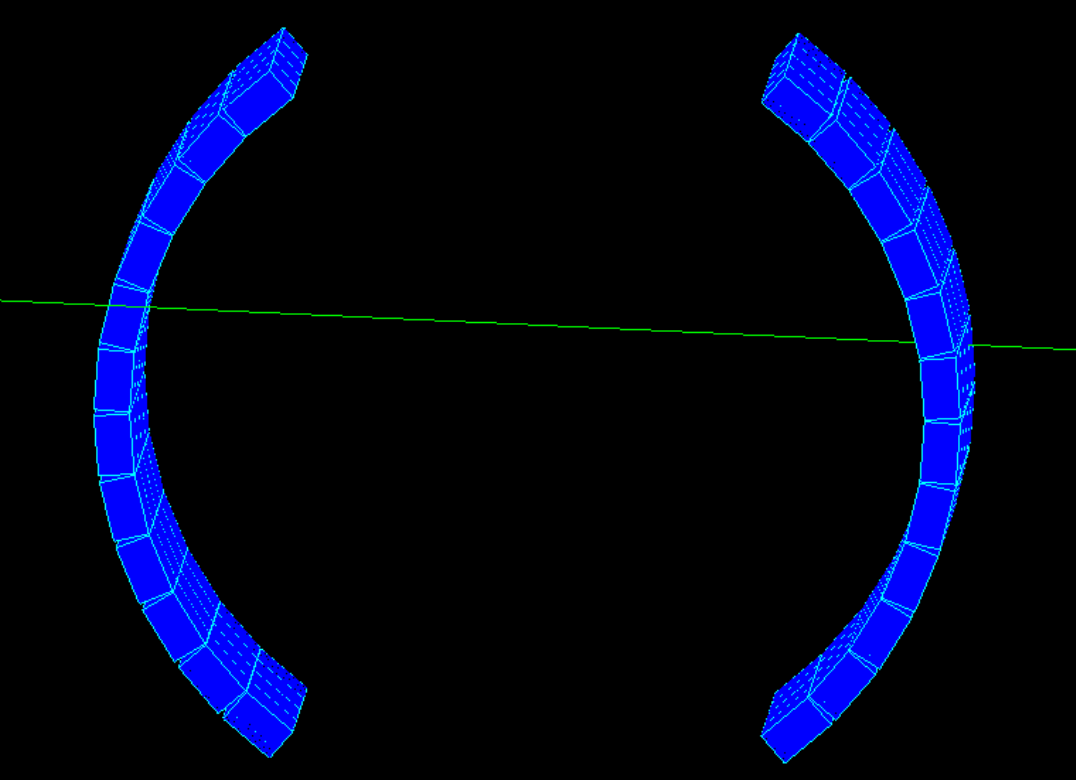
\includegraphics[width=0.5\textwidth]{images/simimage.png}
    \caption{Visualization of crystal detector geometry and single generated back to back gamma in Geant4 using TPPTsim.}

    \label{fig:simimage}
\end{figure}
\newpage
\section{Normalization}

I have separated what we would call normalization into two separate corrections. The first is normalization of the detector and LOR efficiencies, the second is the correction for geometric sensitivity. We approach both with a practical goal of attaining spatial uniformity.

\subsection{Detector Normalization}
Detector normalization aims to normalize the detector efficiencies and therefore the LOR efficiencies, and is done with the component-based approach well established in literature. 

\subsubsection{Forward Model and Iterative Algorithm}
I use a forward model adapted from \cite{componentbasednormalization} which implements component-based normalization. Each LOR efficiency can be modeled as:
\[\epsilon_{i, j} = g_{i,j} \times L_{i} \times R_{j}\]
where $g_{i,j}$ is the target efficiency governed by the source geometry, and $L_{i}$ and $R_{j}$ are the left and right detector efficiencies. In each iteration, we solve for the left arc update ratio $r_i$ by summing the observed counts over all LORs for each left detector, and dividing by the predicted counts, the ratio is multiplied onto the left detector efficiencies for the update. The right arc is updated in a similar way using the new left detector efficiencies. The algorithm alternates between the two arcs to convergence:
\begin{align*}
    1.\quad& r_i^{(k)} = \frac{\sum_j \epsilon_{i, j}}{\sum_j g_{i, j}L_i^{(k)}R_j^{(k)}} \\
    2.\quad& L_{i}^{(k+1)} = L_{i}^{(k)} \times (r_i^{(k)})^{\frac12} \\
    3.\quad& r_j^{(k)} = \frac{\sum_i \epsilon_{i, j}}{\sum_i g_{i, j}L_i^{(k+1)}R_j^{(k)}} \\
    4.\quad& R_{j}^{(k+1)} = R_{j}^{(k)} \times (r_j^{(k)})^{\frac12} \\
\end{align*}
This update step is very sound, it is a form of the general log-likelihood optimization problem, similar to other EM algorithms. I have also included a damping factor of $\frac12$ to prevent the first update step from absorbing the global scale entirely into the left arc, although this is more of an intuitive choice and is mathematically not required. The algorithm converges to the same solution regardless of damping factor given enough iterations.
\newpage
\subsubsection{Data}
The source shape used for normalization should aim to simplify the estimation of $g$ while still populating most LORs. We achieve this with a radius $r=120\text{mm}$ circular scan of a vertically held Ge68 line source, where the source intersects almost all LORs exactly twice (the line source is appropriately approximated as a thin line, it has an active radius of 1.4mm), so that almost all LORs are populated equally. Highly oblique LORs passing outside this cylinder are not populated and therefore excluded from normalization. The data is preprocessed with the previously described cuts. At the time of acquisition, the source has activity $~20.1\text{MBq}$, the source made one full 360 degree scan in 10 minutes, $8.1\text{e}7$ coincidence events were initially recorded, and after all cuts $2.0\text{e}7$ coincidence events remain. The scan path is shown in figure \ref{fig:circpath}.

We also acquire simulation data with the same source shape. 1e9 back to back gammas are generated uniformly in a cylindrical shell between radii 119mm and 121mm and height 110mm centered at isocenter. After grouping and photopeak cuts, 4.15e6 coincidence events are obtained. To validate, we compare the per channel activity 
in figures \ref{fig:circsimhist} and \ref{fig:circsimhm}.

\begin{figure}[H]
    \centering
    \begin{subfigure}{0.9\textwidth}
        \centering
        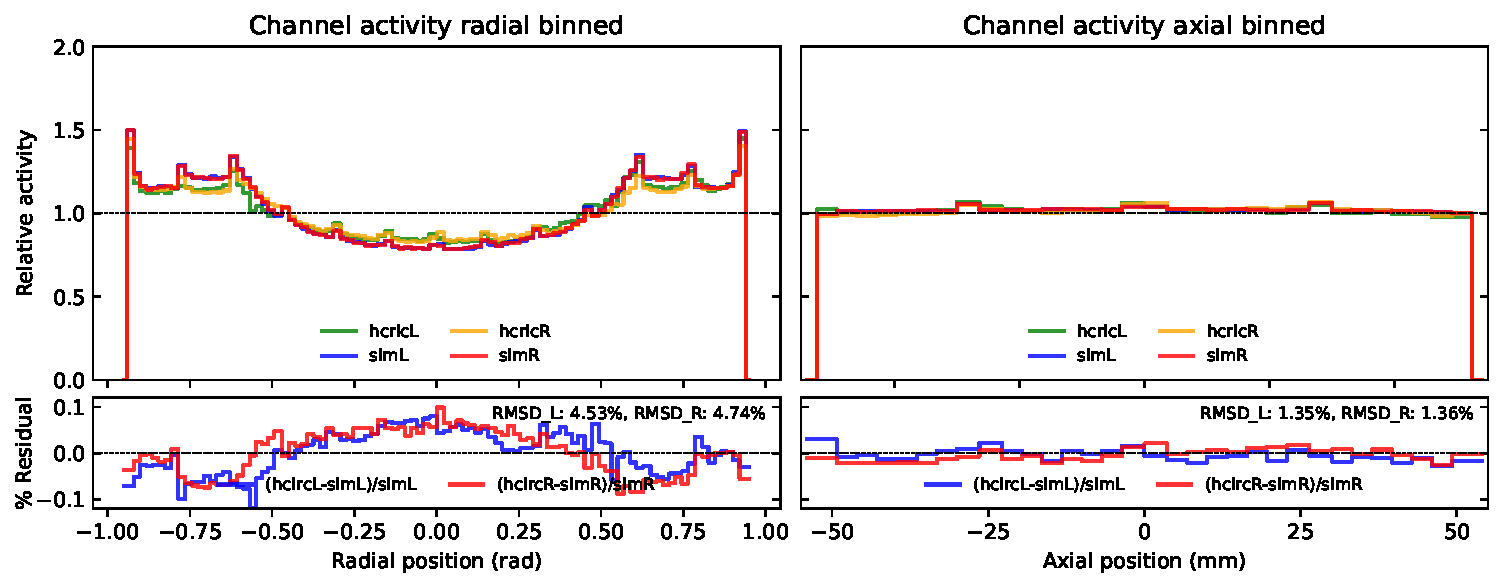
\includegraphics[width=\textwidth]{plots/activityhist/simp.pdf}
        \caption{Circular scan source, photopeak cuts only, compared to simulation.}
    \end{subfigure}
    \begin{subfigure}{0.9\textwidth}
        \centering
        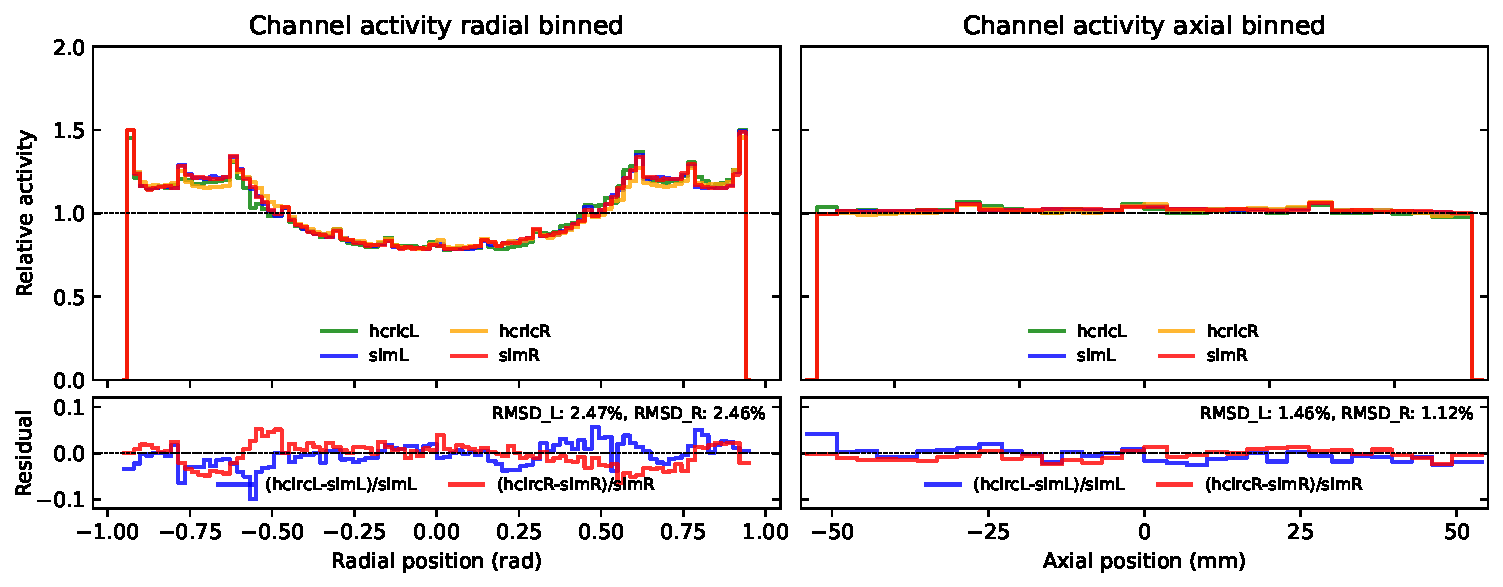
\includegraphics[width=\textwidth]{plots/activityhist/simpgd.pdf}
        \caption{Circular scan source, all cuts, compared to simulation.}
    \end{subfigure}
    \caption{Comparison of channel activity histograms along radial profile and axial profile, normalized to center, with percent residual and simple RMSD calculated. (Top) circular scan source, photopeak cuts only, compared to simulation. (Bottom) circular scan source, all cuts, compared to simulation. We see overall good agreement with all cuts, nice validation of not only the simulation but also the preprocessing cuts. The geometric and duplicate cuts remove most of the residual pattern in the radial profile. Large dips appear in rows or columns containing dead channels.} 
    \label{fig:circsimhist}
\end{figure}


\begin{figure}[H]
    \centering
    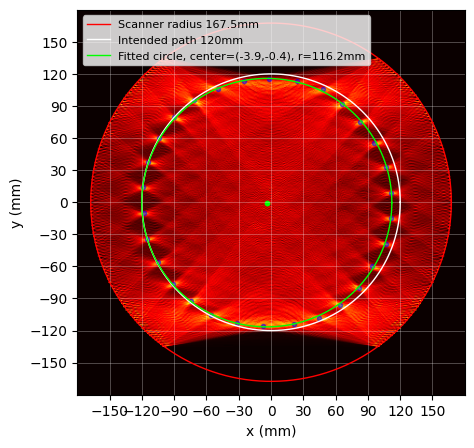
\includegraphics[width=0.5\textwidth]{images/circpath.png}
    \caption{Basic 2D Siddon projection of the circular scan path at 30 second intervals with 1 second windows. All projections normalized and plotted together, arbitrary scale. The maximum activity position for each projection is recorded (plotted blue dots), and fitted to estimate the true path of the source (green line). We see some offset from the intended path, probably need to retake the data. We keep this in mind for now, it may help to explain some asymmetry we later encounter.}
    \label{fig:circpath}
\end{figure}



\begin{figure}[H]
    \centering
    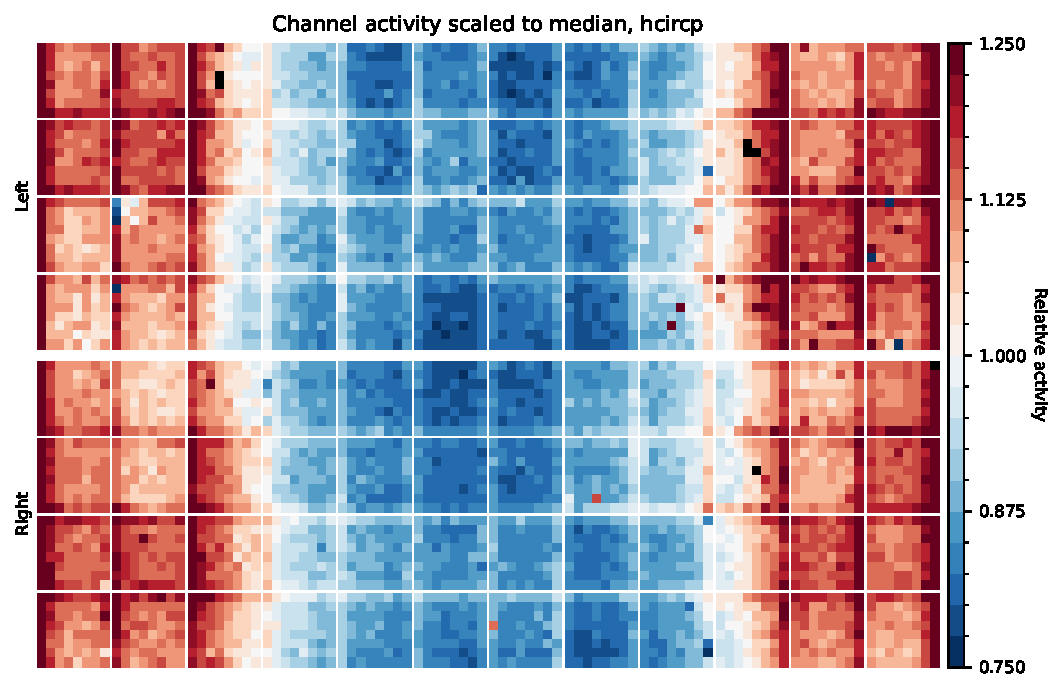
\includegraphics[width=0.45\textwidth]{plots/activityhist/hcircphm.pdf}
    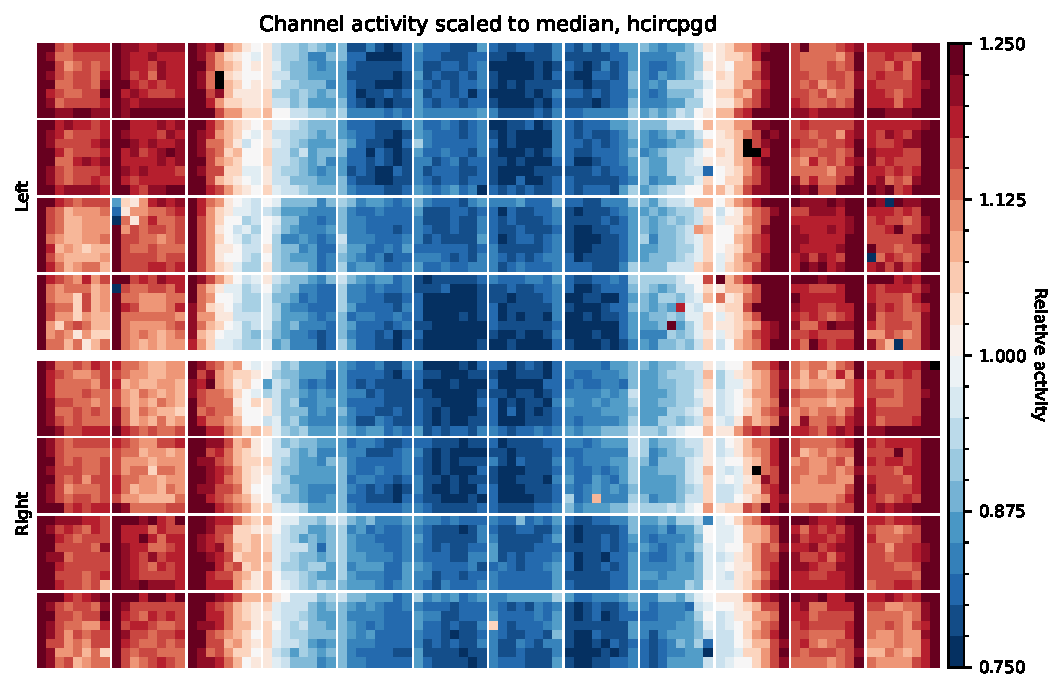
\includegraphics[width=0.45\textwidth]{plots/activityhist/hcircpgdhm.pdf}
    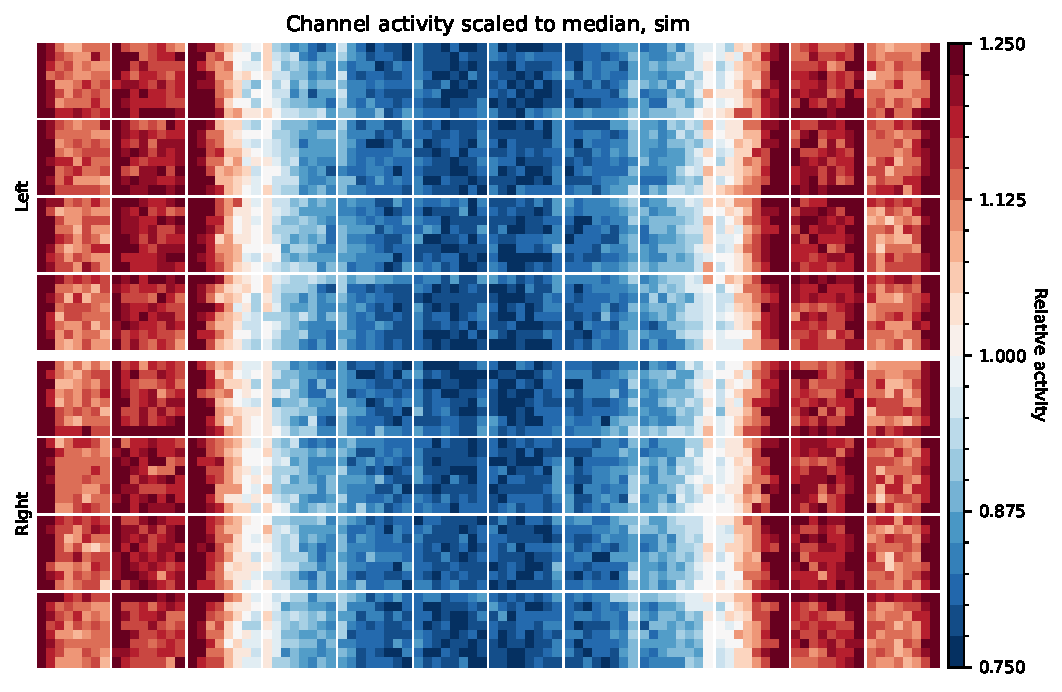
\includegraphics[width=0.45\textwidth]{plots/activityhist/simhm.pdf}
    \caption{Channel activity heatmaps scaled to median for: (upper left) circular scan source, photopeak cuts only, (upper right) circular scan source, all cuts, (lower) simulation.}
    \label{fig:circsimhm}
\end{figure}


\subsubsection{Computing $g$}

$g$ is the target efficiency matrix, it describes the expected LOR response given some source geometry. For perfect $g$ characterization, we would need unrealistic statistics to populate every LOR. To get around this, $g$ is commonly factored into radial, axial, block, etc. factors which each exploit some symmetry in the geometric sensitivity, allowing events to be pooled into a much smaller number of bins. For TPPT, we can implement a simple factorization into only radial and axial factors, into which we allow other geometric effects to be absorbed.

In TPPT we have 3072 detectors on each arc, aranged into 96 radial (xy) positions and 32 axial (z) positions on each arc. A simple binning scheme might be to pool all events into one of $96\times96 = 9216$ radial factors (here a factor is a left and right position pairing) and into one of $32\times32 = 1024$ axial factors, then constructing $g$ by multiplying the approprate radial and axial factor for each LOR, assuming the radial and axial factors are roughly separable. This reduces the number of total response bins from $3072^2$ to $96^2 + 32^2$, which is more statistically robust. 

However, many implementations in literature further exploit certain symmetries in the LOR geometry to enforce symmetry in $g$ where it is expected to exist in order to generalize the behavior of LORs which are geometrically identical. For example, another binning scheme could be to pool events into axial factors defined by angle instead of xy pairing. However, in TPPT we don't have full rotational symmetry, and we enforce bipartite coincidence grouping, so many LORs that would exist in a full ring scanner do not exist in TPPT, which would lead angular binning to require additional corrections. Instead, I implement a symmetrization based on reflection symmetry; each radial pairing is binned together with its up to 3 other reflections in xy, $(\pm y_L, \pm y_R)$, each $y$ has unique $x$; each axial pairingis binned together with its up to 3 other reflections in z, $(\pm z_L, \pm z_R)$. The average of the contributing pairs in each bin is then used to construct $g$. This way we can still achieve some symmetrization, while still ensuring that the LORs in each bin are geometrically identical.

\begin{figure}[H]
    \centering
    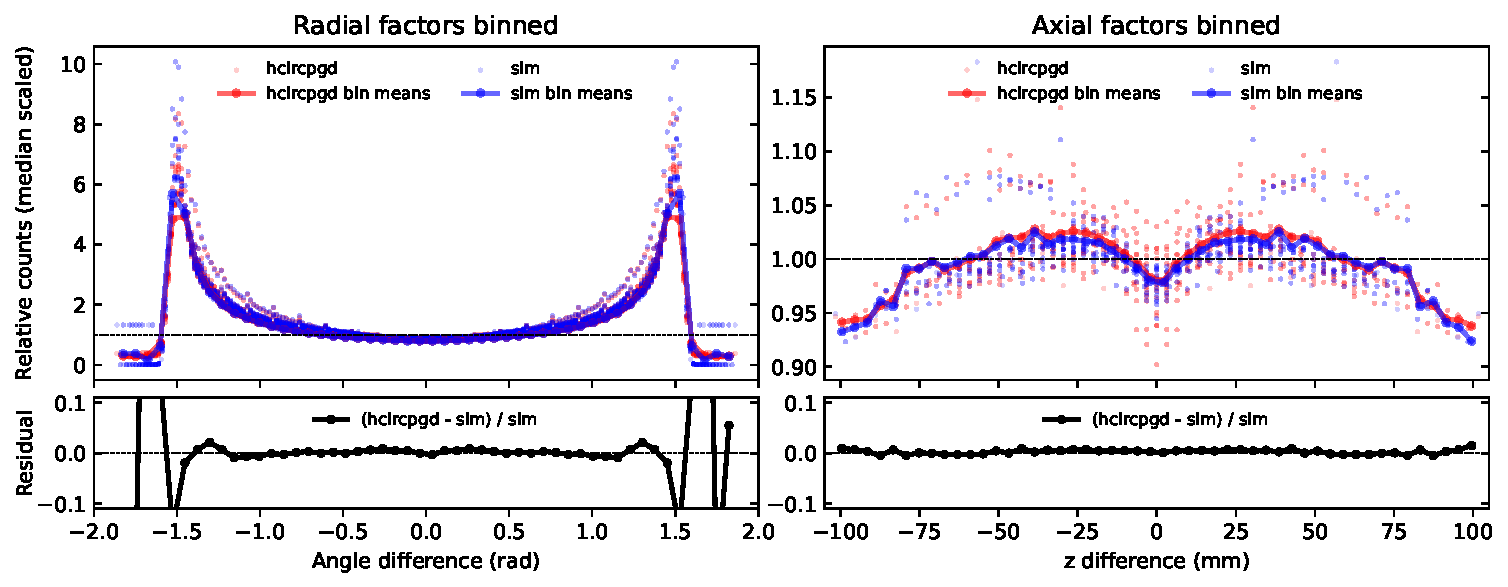
\includegraphics[width=0.9\textwidth]{plots/radialaxialfactors.pdf}
    \caption{Comparison of radial and axial factors computed from real and simulated data. Both individual factor-count points and bin means are plotted. We see essentially the same behavior for both within relevant angular region. Angle difference refers to the angular difference in crystal orientation of the two radial groups each radial factor connects. z difference is defined similarly. ``Bin means'' are computed by averaging the radial or axial factors when binned into 50 angle difference or z difference bins. At large angles, LORs no longer intersect the source, leading to a dropoff and mismatched behavior between real and simulated data as real data still measures some activity in these empty regions.}
    \label{fig:g_factors}
\end{figure}

\newpage
\subsubsection{Algorithm Convergence}
We expect the algorithm to find converging solutions for $L_i$ and $R_j$. Figure \ref{fig:convergence} shows heatmaps of channel activity corrected for $g$ and accompanying histogram for the channel distributions. Plots for all iterations are available in plots/convergence/.

\begin{figure}[H]
    \centering
    \begin{subfigure}{\textwidth}
        \centering
        \begin{tabular}{cc}
            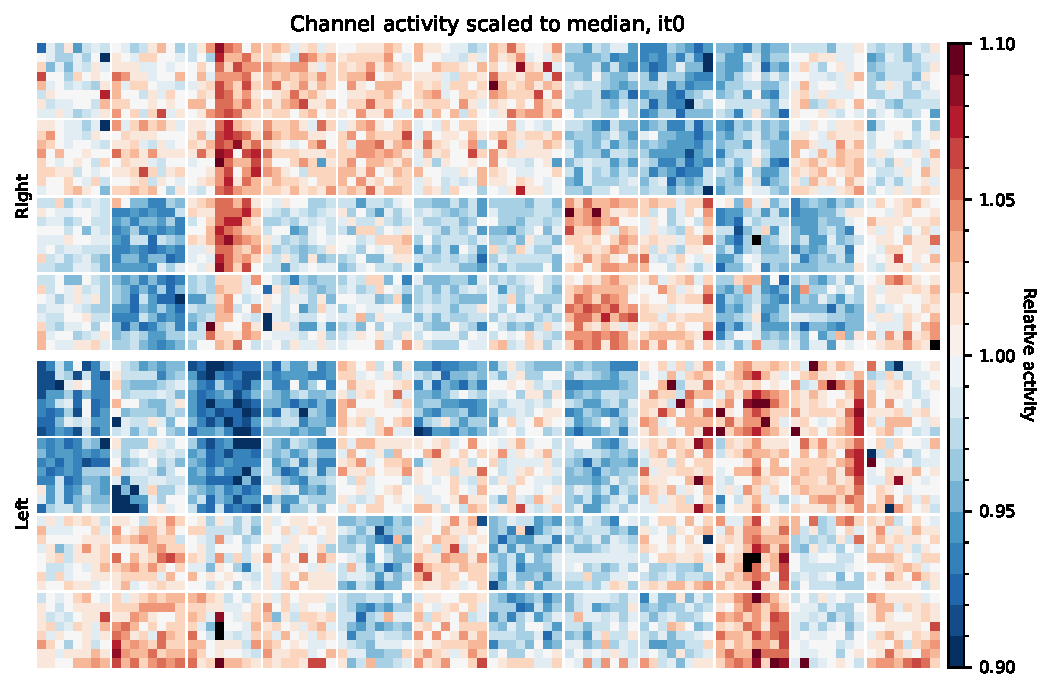
\includegraphics[width=0.45\textwidth]{plots/convergence/Channel activity scaled to median, it0.pdf} &
            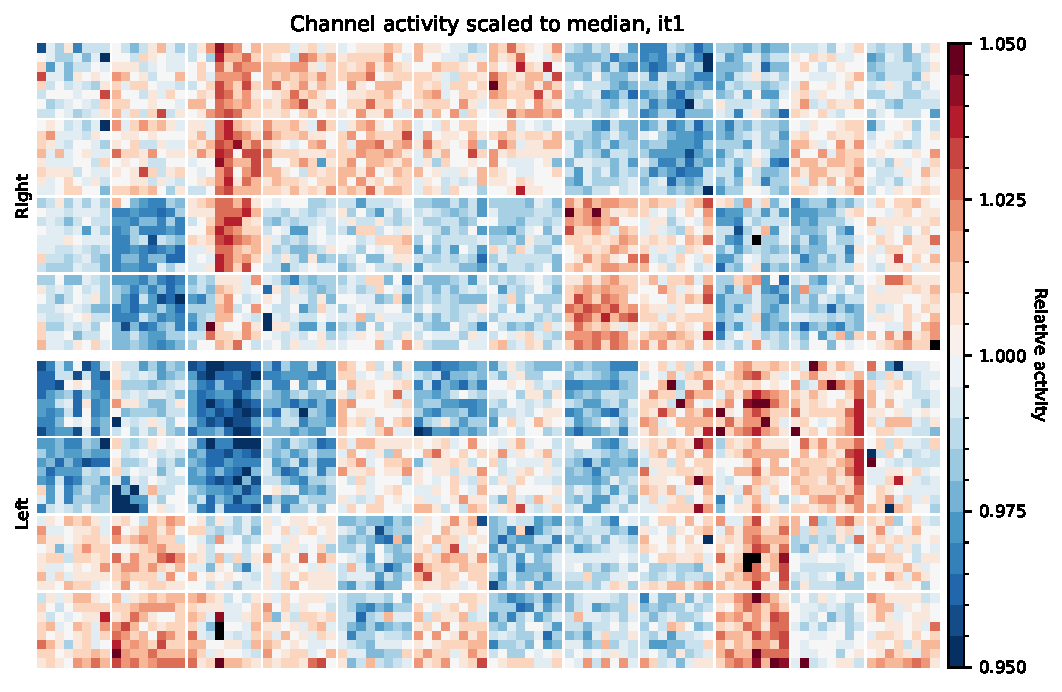
\includegraphics[width=0.45\textwidth]{plots/convergence/Channel activity scaled to median, it1.pdf} \\
            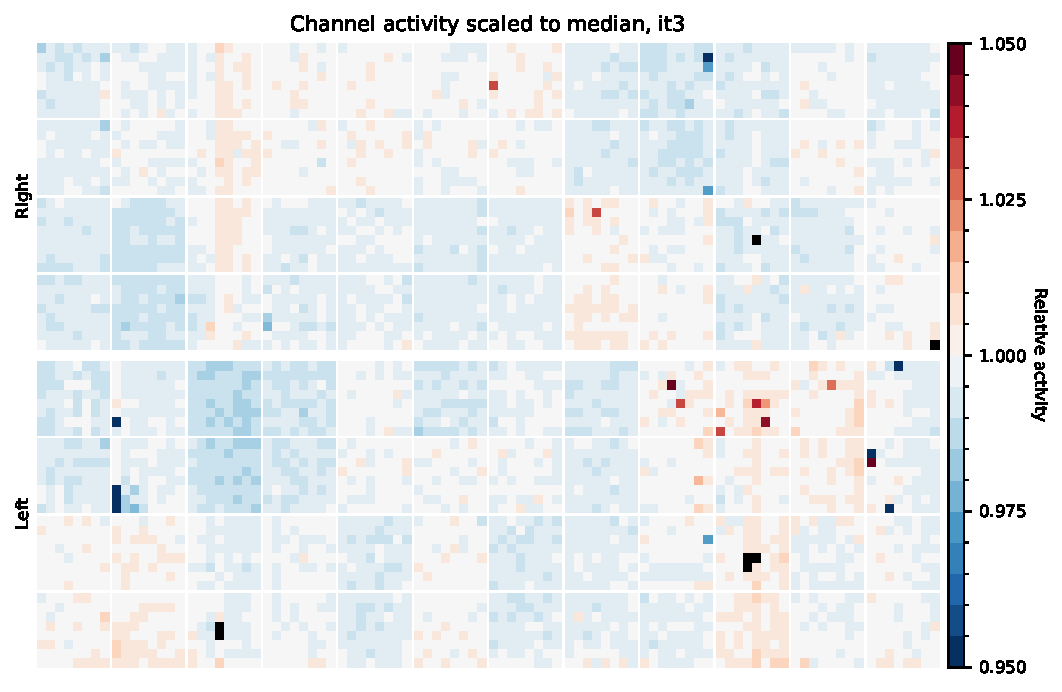
\includegraphics[width=0.45\textwidth]{plots/convergence/Channel activity scaled to median, it3.pdf} &
            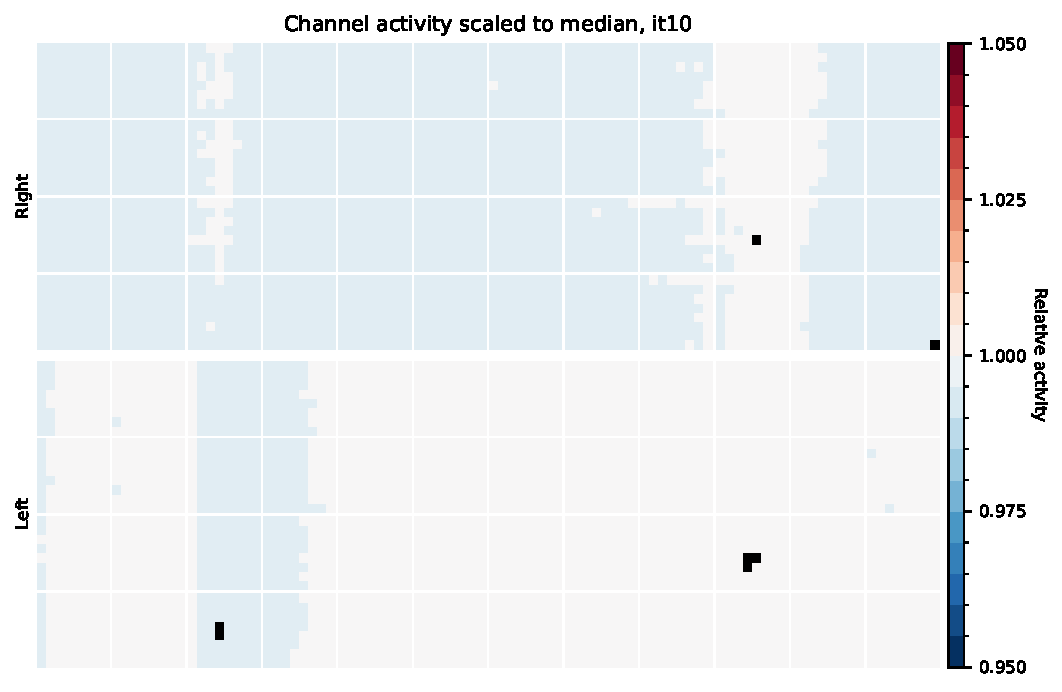
\includegraphics[width=0.45\textwidth]{plots/convergence/Channel activity scaled to median, it10.pdf}
        \end{tabular}
        \caption{Channel activity heatmaps scaled to median for iterations 0 (no normalization), 1, 3, and 10, each corrected $g$.}
    \end{subfigure}
    \begin{subfigure}{\textwidth}
        \centering
        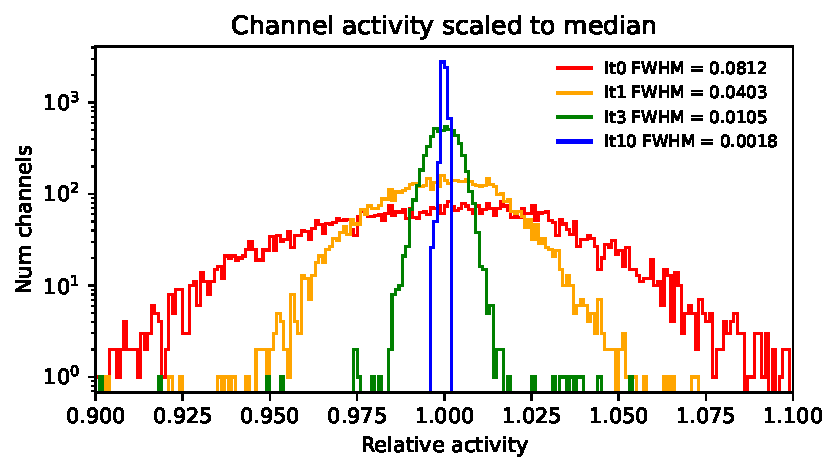
\includegraphics[width=0.6\textwidth]{plots/convergence/histselectediterations.pdf}
        \caption{Corresponding channel activities histogrammed for each iteration.}
    \end{subfigure}
    \caption{Channel activity convergence, shows expected behavior of algorithm. Some residual effect remains, possibly due to source shape error or missing counts from opposite arc dead channels.}
    \label{fig:convergence}
\end{figure}

\newpage
\subsection{Geometric Sensitivity}
We have been using the CASToR \cite{castor} implementation of the MLEM algorithm for listmode PET reconstruction with Joseph projector. The standard MLEM algorithm is given in various forms in literature \cite{mlemalgorithm} \cite{tof_mlem_jpet},  generally it looks like:
\[f_j^{(k+1)} = \frac{f_j^{(k)}}{S_j} \sum_i\frac{a_{ij}}{\sum_{j'}a_{ij'}f_{j'}^{(k)}+b_i}\]
Where $f_j^{(k)}$ is the activity estimate of voxel $j$ at iteration $k$, $a_{ij}$ is the probability contribution of the measurement $i$ to the voxel $j$, $b_i$ is an estimated background from scatters, randoms, etc., and $S_j$ is the sensitivity image:
\[S_j = \sum_i a_{ij}\]
The normalization factors appear as part of the probability contribution $a_{ij}$, and is the same for a single LOR. So $a_{ij}$ becomes the product of the normalization factor and the pure probability of a measurement $i$ contributing to voxel $j$:
\[a_{ij} = n_i P_{ij}\]
When we include normalization, both the update step and the sensitivity image are impacted. What we observe is that this is not enough to correct for spatial uniformity, as the sensitivity is not well modeled due to non-full scanner geometry of TPPT. Thus we need a more robust estimate for the geometric sensitivity $S$.
\subsubsection{Simulating $S$}
To obtain a more accurate estimate for $S$, 1e9 back to back 511keV gamma pairs were generated uniformly in a 160mm radius and 110mm height cylinder centered at the isocenter, with random direction and no acollinearity. Only the scintillator detector geometry is used to obtain an ideal, non-scattered sensitivity image. I allow Geant4 to simulate interaction physics, allow TPPTsim to collect deposited energy per event, use TPPTbuilder to generate detector-like singles, and use TPPTcoinc for coincidence grouping and photopeak cuts. I set the energy window to $(0.85, 1.15)\times511\text{keV}$ to roughly match our 2.5$\sigma$ photopeak window at approximately $8.2\%$ energy resolution used in our photopeak cuts on real data. 4.2e6 coincidence events were recorded after grouping and photopeak cuts. Recorded coincidences are binned into 1mm voxels and symmetrized.

The sensitivity image computed for ray-based projectors such as Joseph $S_{J}$ are separable into a local LOR granularity and a broad regional sensitivity. We cannot supply $S_{MC}$ directly into the MLEM algorithm because it is only a measure of the broad sensitivity. Instead, we can isolate the broad sensitivity of $S_{J}$ by convolving in a similar manner as we did for $S_{MC}$ and find the ratio of the broad sensitivity $S'_{J}$ to $S_{MC}$. Then this ratio is multiplied back onto $S_{J}$ to obtain the corrected sensitivity image, which is supplied to the MLEM algorithm. Sensitivity images are shown in figure \ref{fig:sensitivity_image}.

\begin{figure}[H]
    \centering
    \begin{tabular}{cc}
        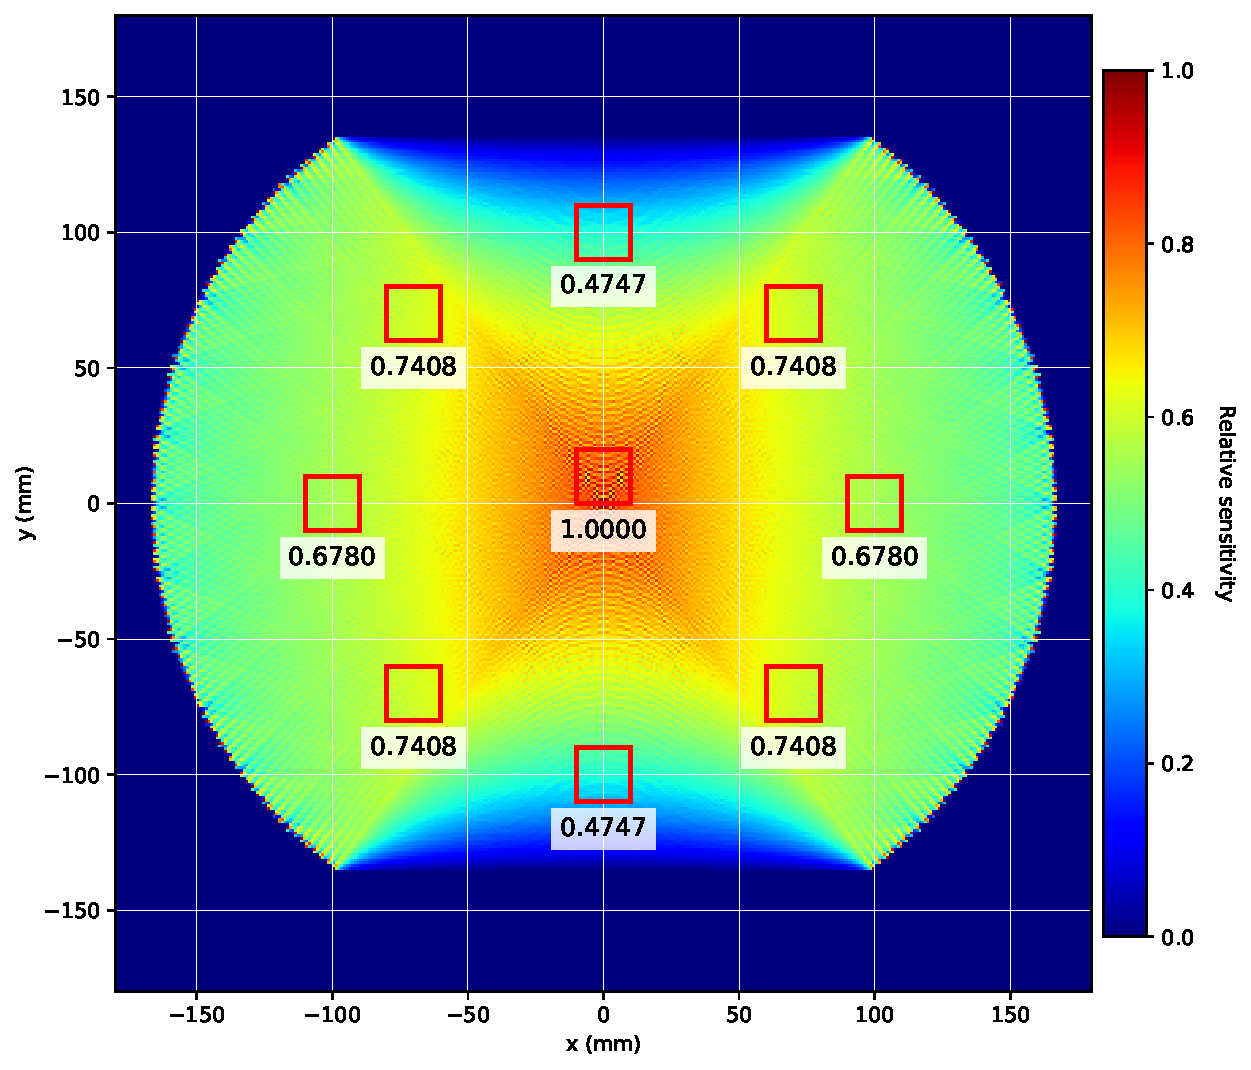
\includegraphics[width=0.45\textwidth]{plots/sensimgs/sensjosephbipartite.pdf} &
        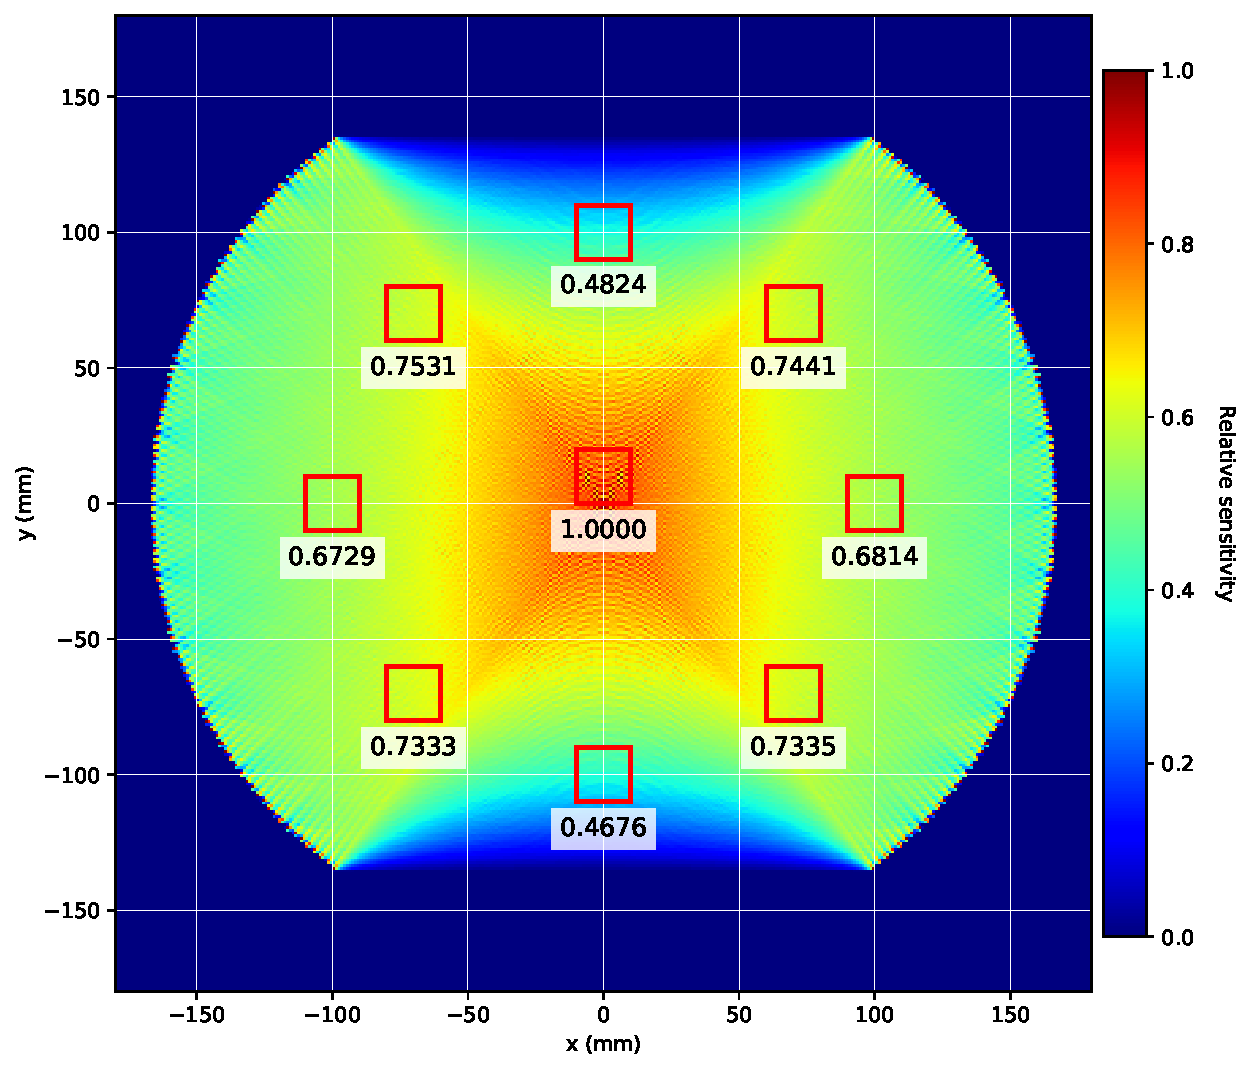
\includegraphics[width=0.45\textwidth]{plots/sensimgs/sensjosephbipartiten.pdf} \\
        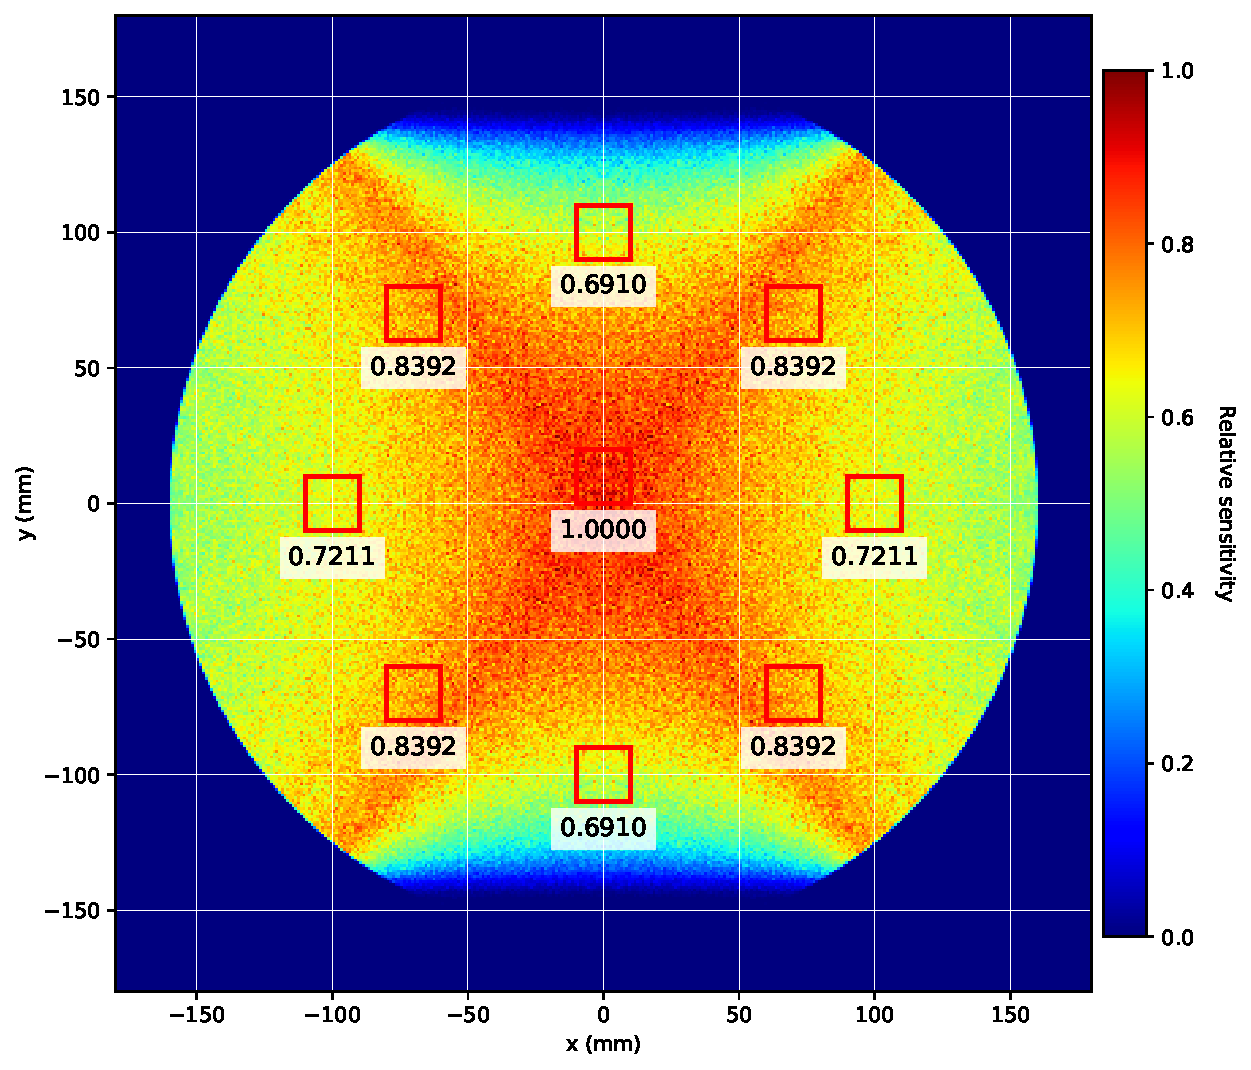
\includegraphics[width=0.45\textwidth]{plots/sensimgs/mc3d.pdf} &
        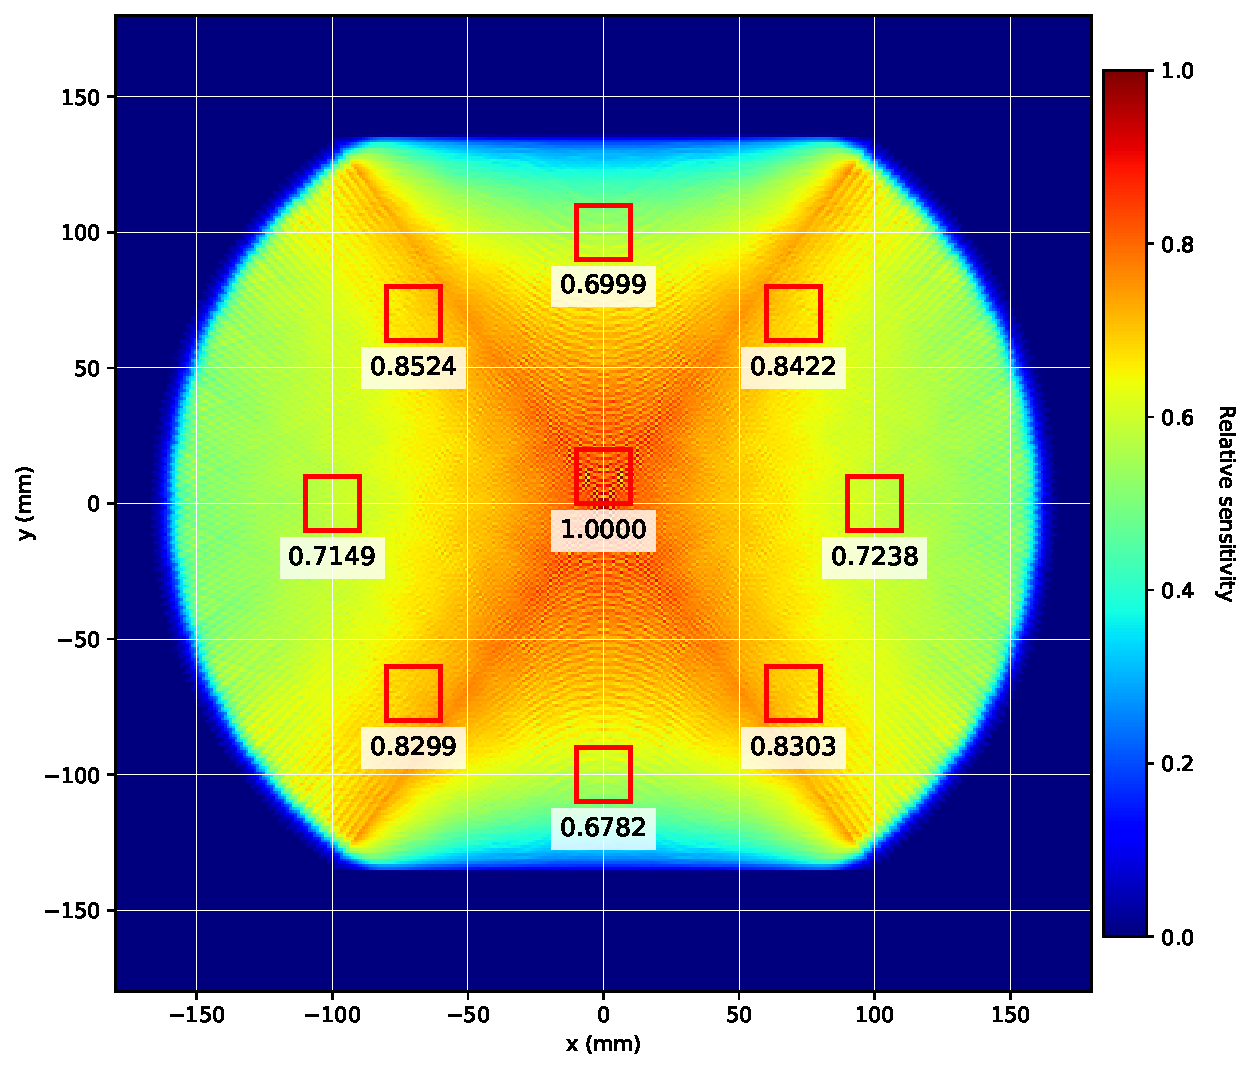
\includegraphics[width=0.45\textwidth]{plots/sensimgs/correctedimg.pdf} \\
    \end{tabular}
    \caption{Sensitivity images collapsed onto transverse view. (top left) Sensitivity image from only Joseph projection ($S_J = \sum_i P_{ij}$); (top right) Sensitivity image from Joseph projection with normalization ($S_{Jn} = \sum_i n_i P_{ij}$); (bottom left) Recorded coincidence events binned by generation position into 1mm voxels and symmetrized across $\pm x$, $\pm y$, and $\pm z$ ($S_{MC}$); (bottom right) Corrected sensitivity image obtained from gaussian convolution of $S_{MC} / S_J$ and multiplied onto $S_{Jn}$, this is what is fed into CASToR. 9 regions representing the locations of the 9 points used for spatial resolution testing are shown in red boxes, the mean sensitivity in each region is given relative to the central region.}
    \label{fig:sensitivity_image}
\end{figure}
\newpage
\subsection{Quantitative Validation}
Without a uniform phantom, we can test uniformity by reconstructing the line source at different locations in the scanner, here specifically we use a point 1cm in the $+y$ direction from the isocenter and 8 points at a 10cm radius from the center. We typically use these runs to test for spatial resolution, but we can also use them as a rough test for uniformity. Example reconstructions without normalization and sensitivity correction are shown in figure \ref{fig:uniformity}, and with normalization and sensitivity correction are shown in figure \ref{fig:uniformity_normalized}.


\begin{figure}[H]
    \centering
    \begin{tabular}{ccc}
        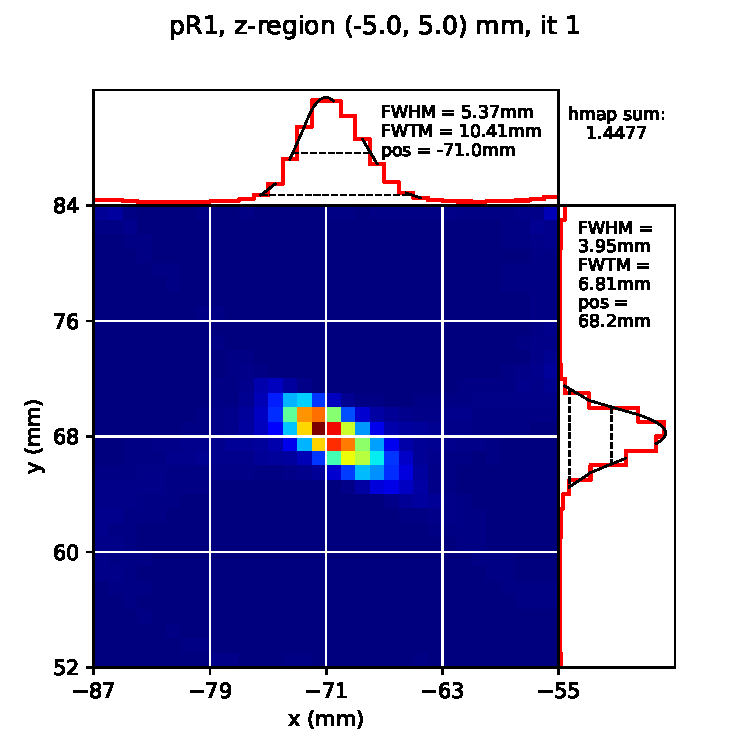
\includegraphics[width=0.3\textwidth]{plots/spatialresolution/pR11_xy_it1_spatialresolution.pdf} &
        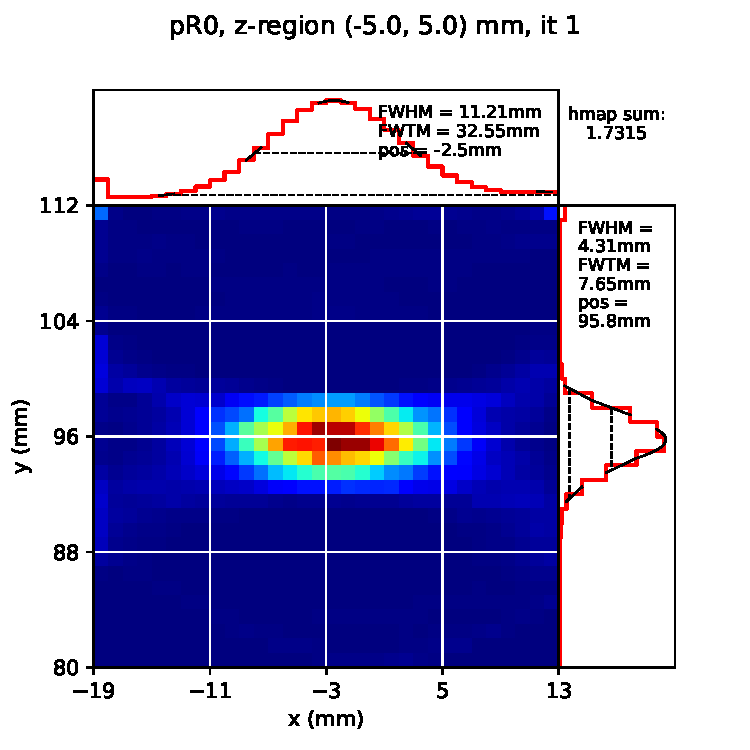
\includegraphics[width=0.3\textwidth]{plots/spatialresolution/pR01_xy_it1_spatialresolution.pdf} &
        \includegraphics[width=0.3\textwidth]{plots/spatialresolution/pr71_xy_it1_spatialresolution.pdf} \\
        \includegraphics[width=0.3\textwidth]{plots/spatialresolution/pr21_xy_it1_spatialresolution.pdf} &
        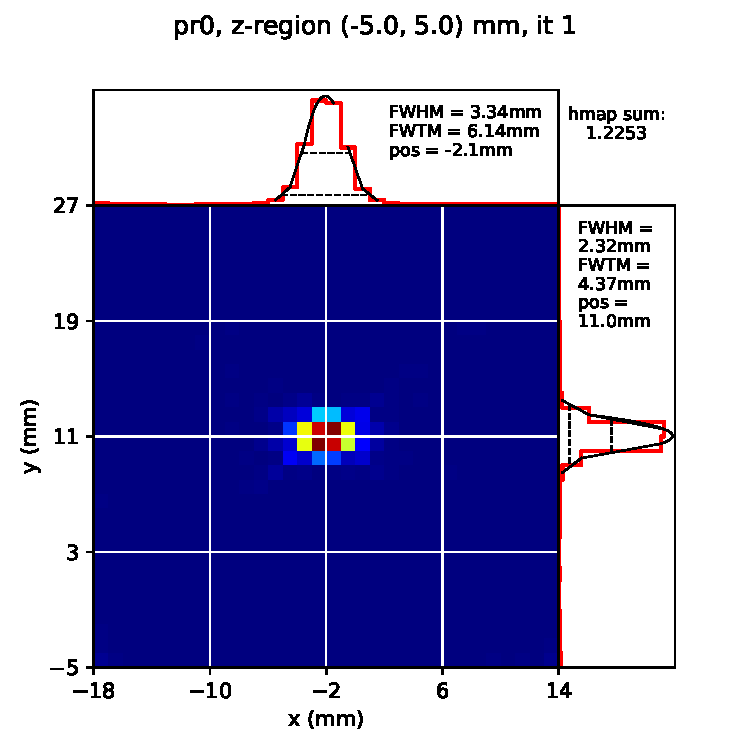
\includegraphics[width=0.3\textwidth]{plots/spatialresolution/pr01_xy_it1_spatialresolution.pdf} &
        \includegraphics[width=0.3\textwidth]{plots/spatialresolution/pr61_xy_it1_spatialresolution.pdf} \\
        \includegraphics[width=0.3\textwidth]{plots/spatialresolution/pr31_xy_it1_spatialresolution.pdf} &
        \includegraphics[width=0.3\textwidth]{plots/spatialresolution/pr41_xy_it1_spatialresolution.pdf} &
        \includegraphics[width=0.3\textwidth]{plots/spatialresolution/pr51_xy_it1_spatialresolution.pdf}
    \end{tabular}
    \caption{Example MLEM single iteration reconstructions of the line source at different locations in the scanner, no smoothing, integrated over a 10mm slice centered at $z=0$. A heatmap sum of the voxel values shown is reported, without any thresholding or other image processing, these are arbitrary units. We see that the activity depends strongly on the location of the source, clear differences between center, corner, top/bottom, and left/right positions. A simple coefficient of variation for these 9 positions is computed as $\sigma/\mu = 0.101$.}
    \label{fig:uniformity}
\end{figure}

\begin{figure}[H]
    \centering
    \begin{tabular}{ccc}
        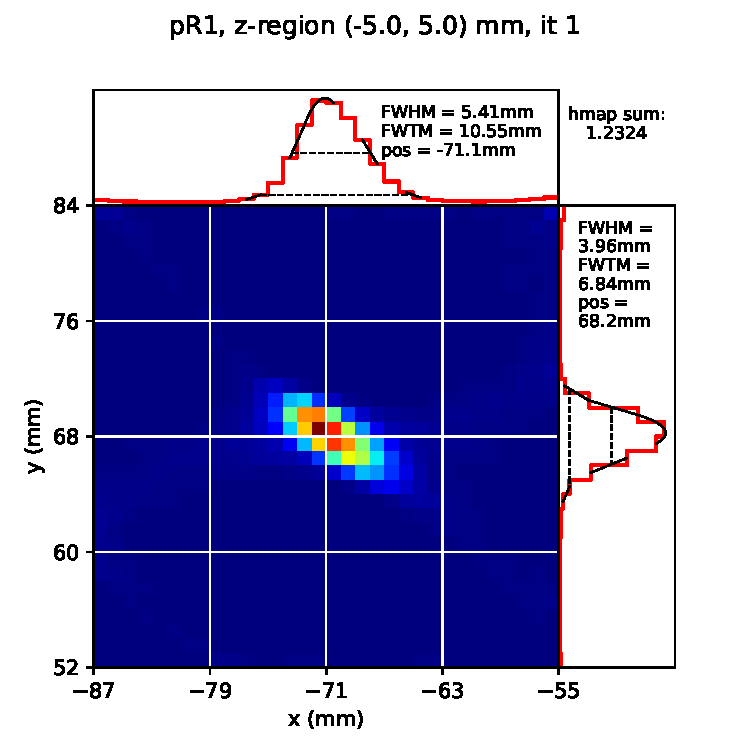
\includegraphics[width=0.3\textwidth]{plots/spatialresolution/pR11ns_xy_it1_spatialresolution.pdf} &
        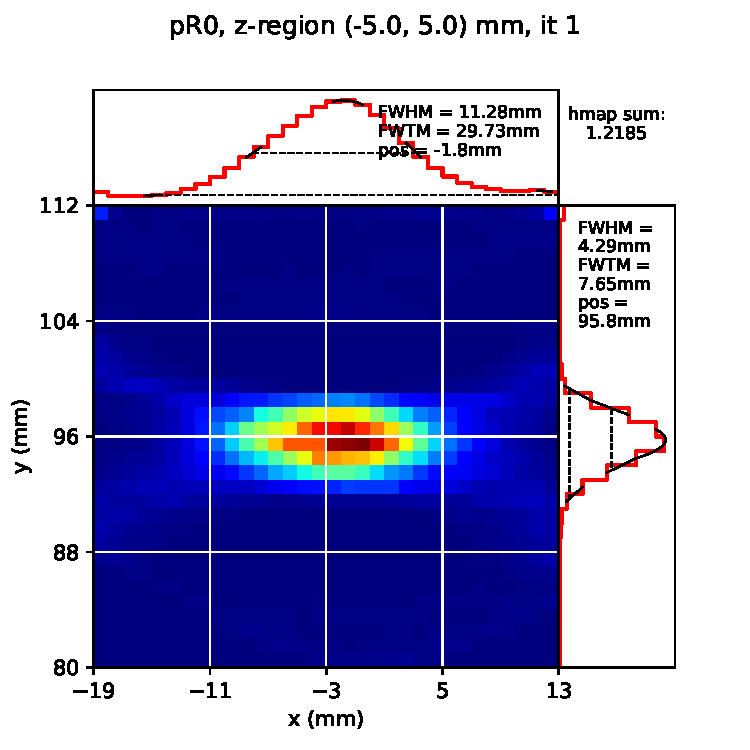
\includegraphics[width=0.3\textwidth]{plots/spatialresolution/pR01ns_xy_it1_spatialresolution.pdf} &
        \includegraphics[width=0.3\textwidth]{plots/spatialresolution/pr71ns_xy_it1_spatialresolution.pdf} \\
        \includegraphics[width=0.3\textwidth]{plots/spatialresolution/pr21ns_xy_it1_spatialresolution.pdf} &
        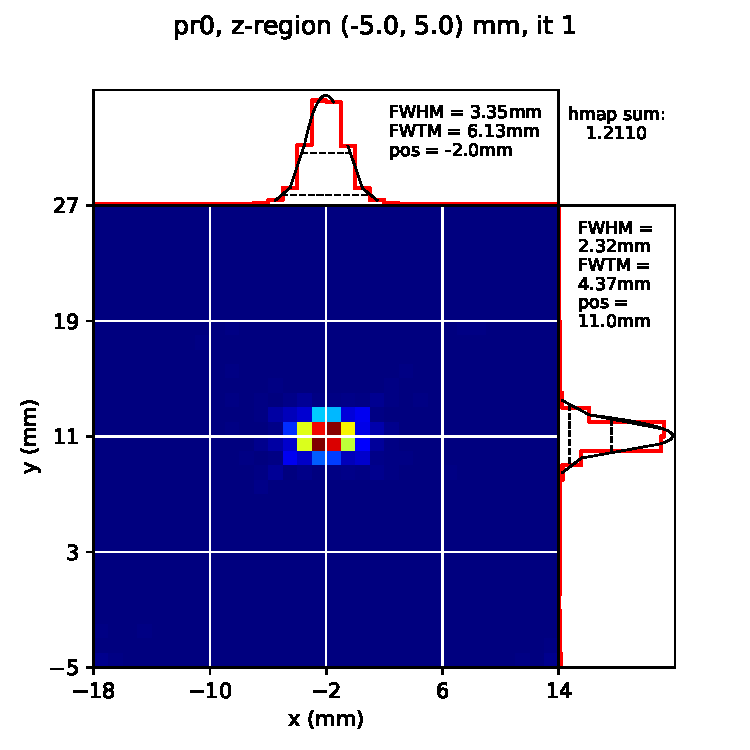
\includegraphics[width=0.3\textwidth]{plots/spatialresolution/pr01ns_xy_it1_spatialresolution.pdf} &
        \includegraphics[width=0.3\textwidth]{plots/spatialresolution/pr61ns_xy_it1_spatialresolution.pdf} \\
        \includegraphics[width=0.3\textwidth]{plots/spatialresolution/pr31ns_xy_it1_spatialresolution.pdf} &
        \includegraphics[width=0.3\textwidth]{plots/spatialresolution/pr41ns_xy_it1_spatialresolution.pdf} &
        \includegraphics[width=0.3\textwidth]{plots/spatialresolution/pr51ns_xy_it1_spatialresolution.pdf}
    \end{tabular}
    \caption{Same reconstructions but with normalization and geometric sensitivity correction applied. Simple coefficient of variation for these 9 positions is computed as $\sigma/\mu = 0.017$, which is a significant improvement. Some residual non-uniformity is still present, possibly due to imperfect source shape.}
    \label{fig:uniformity_normalized}
\end{figure}

The reconstructed activities before and after normalization and sensitivity correction are tabulated here, relative to the center.
\begin{table}[H]
    \centering
    \begin{tabular}{c|cccccccccc}
        & pr0 & pR0 & pR1 & pR2 & pR3 & pR4 & pR5 & pR6 & pR7 & $\mu/\sigma$ \\
        \hline
        Unnormalized & 1.0000 & 1.3902 & 1.1674 & 1.1399 & 1.2006 & 1.3879 & 1.1943 & 1.1186 & 1.1689 & 0.1013 \\
        Normalized & 1.0000 & 1.0062 & 1.0177 & 1.0497 & 1.0455 & 0.9981 & 1.0268 & 1.0095 & 1.0217 & 0.0172    
    \end{tabular}
\end{table}

\newpage
\section{Time Alignment}
Time alignment corrects for LOR time offsets, which we want to all be zero modulo geometry.

\subsection{Forward Model and Iterative Algorithm}
We use the forward model for LOR time offsets
\[\Delta t_{i, j} = g_{i, j} + L_i - R_j\]
where $g_{i, j}$ is the target offset, and $L_i$ and $R_j$ are the left and right detector time offsets. A very similar forward model is used in \cite{timingoffset}.

In each iteration, we solve for the left arc updates by histogramming the observed time differences for each LOR, corrected for the predicted time offset, and computing a residual $r_i$ between the observed and predicted time differences via gaussian fitting of the timing distribution. The residual is added to the left detector time offsets for the update. The right arc is updated in a similar way using the new left detector time offsets, and the algorithm alternates between the two arcs to convergence:
\begin{align*}
    1.\quad& r_i^{(k)} = (\Delta t_{i, j} - g_{i, j}) - L_i^{(k)} + R_j^{(k)} \\
    2.\quad& L_{i}^{(k+1)} = L_{i}^{(k)} + \frac12r_i^{(k)} \\
    3.\quad& r_j^{(k)} = (\Delta t_{i, j} - g_{i, j}) - L_i^{(k+1)} + R_j^{(k)} \\
    4.\quad& R_{j}^{(k+1)} = R_{j}^{(k)} - \frac12r_j^{(k)} \\
\end{align*}
Again the damping factor of $\frac12$ is an intutive choice and not mathematically required. Originally I actually intended for this damping factor to split the contribution of the offset between the left and right arcs. The choice of sign on $L$ and $R$ comes from our TOF as $(L_i - R_j)c/ 2$.

\subsubsection{Data}
The source used for time alignment should aim to simplify the estimation of the true geometric time offset while still populating most LORs. We achieve this with a scanning source moving in the y-plane at $x=0\text{mm}$ spanning $y=\pm120\text{mm}$. This allows for a straightforward computation of $g$. The scan path is shown in figure \ref{fig:vertpath}.


\subsubsection{Computing $g$}

In time alignment, $g$ is the distance between the midpoint of the LOR and the intersection of the LOR with the $x=0$ plane, converted to picoseconds. This distance is calculated straightforwadly from known geometry of the LOR endpoint detectors. No additional simulation is necessary. When describing a LOR ``module geometry'' or ``corrected for geometry'', what is meant is that $g_{i,j}$ is subtracted from the observed time difference to center it at 0.

\subsection{Algorithm Convergence}

We expect the algorithm to find converging solutions for $L_i$ and $R_j$. Figure \ref{fig:convergence_time_alignment} shows heatmaps of channels with pooled LOR counts and accompanying histograms for the channel distributions. Plots for all iterations are available in plots/timecalconv/.

\begin{figure}[H]
    \centering
    \begin{subfigure}{\textwidth}
        \centering
        \begin{tabular}{cc}
            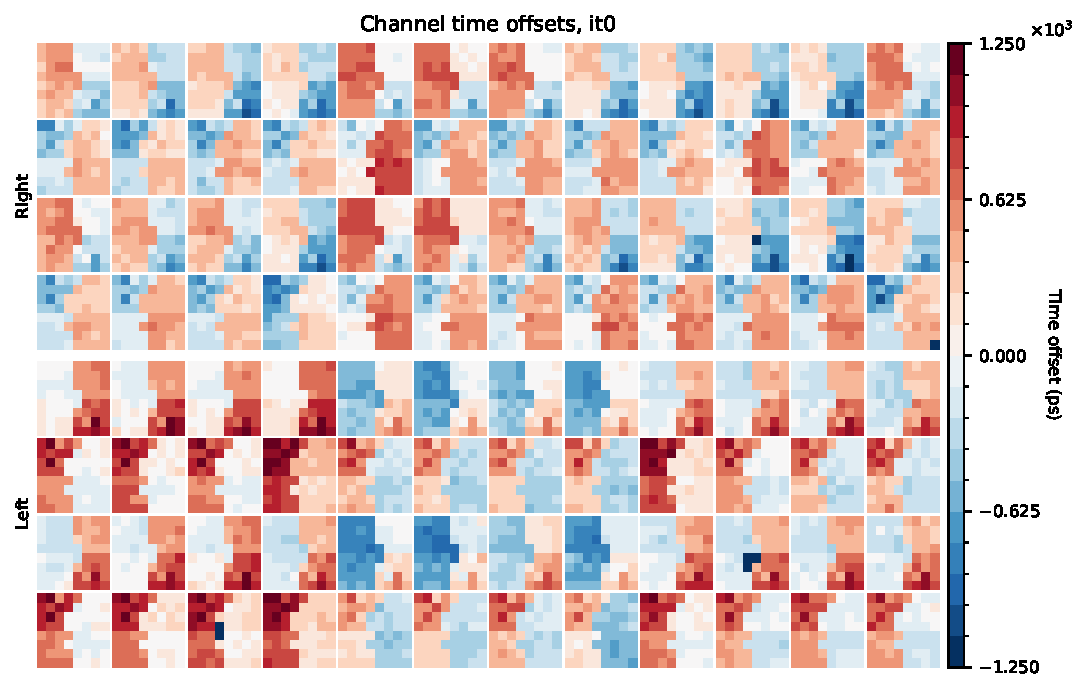
\includegraphics[width=0.45\textwidth]{plots/timecalconv/Channel time offsets, it0.pdf} &
            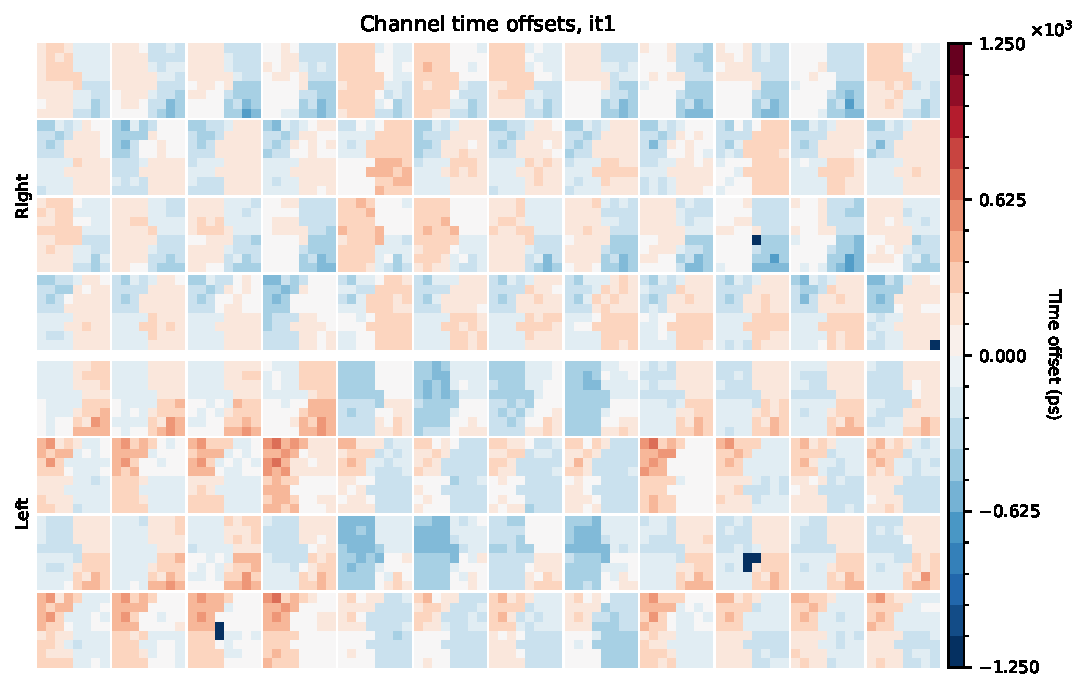
\includegraphics[width=0.45\textwidth]{plots/timecalconv/Channel time offsets, it1.pdf} \\
            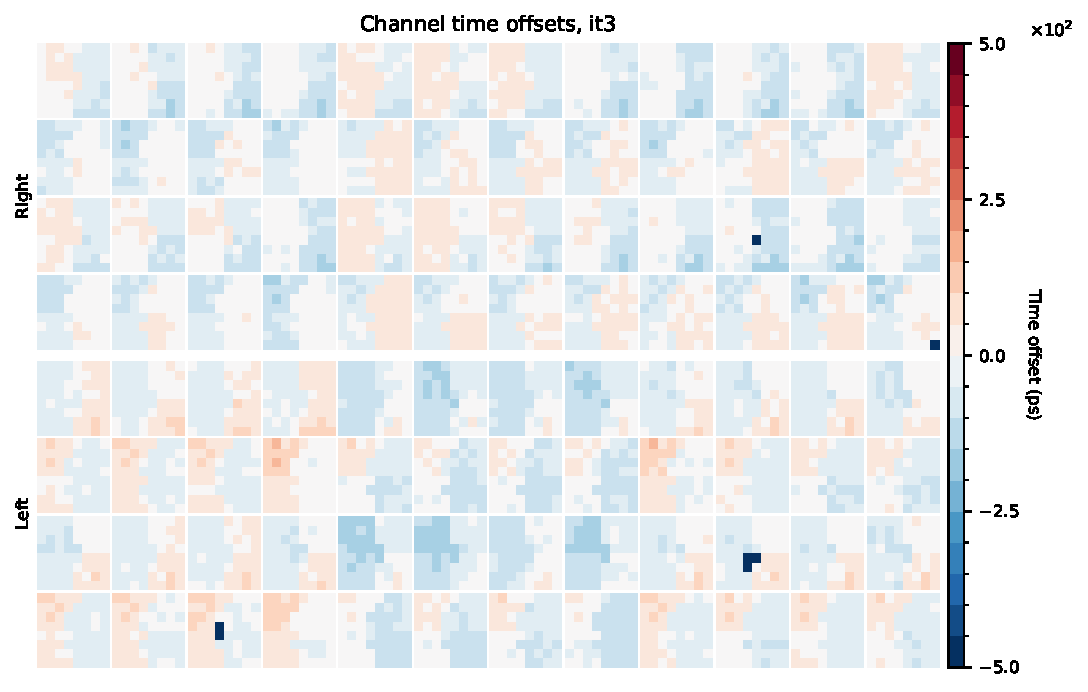
\includegraphics[width=0.45\textwidth]{plots/timecalconv/Channel time offsets, it3.pdf} &
            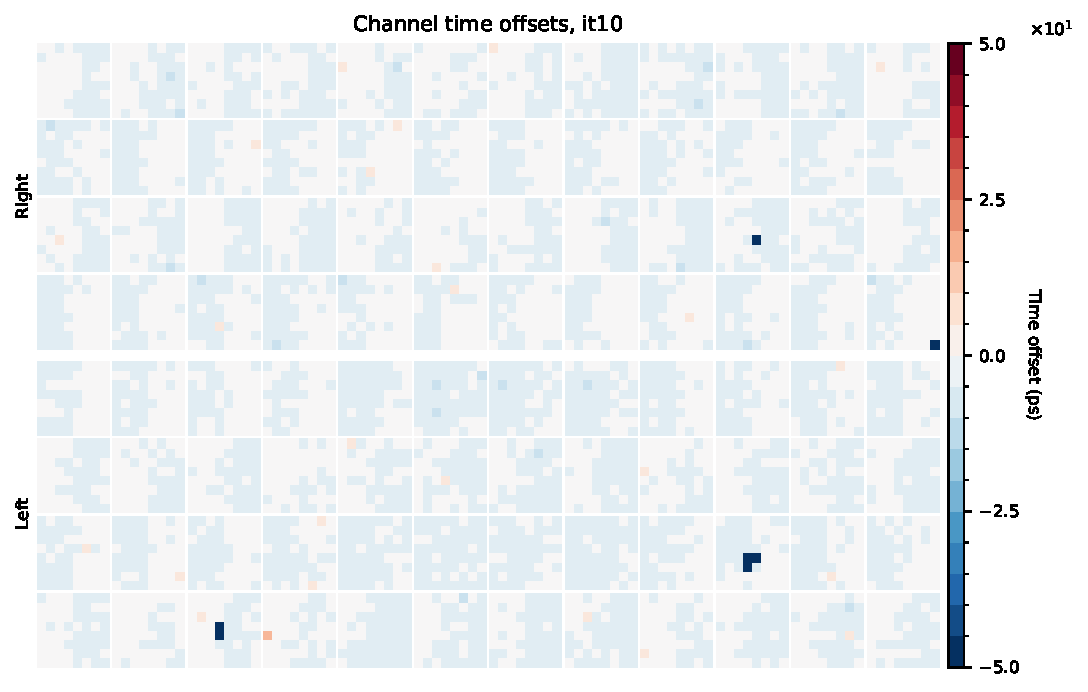
\includegraphics[width=0.45\textwidth]{plots/timecalconv/Channel time offsets, it10.pdf}
        \end{tabular}
        \caption{Channel time offset heatmaps for iterations 0, 1, 3, and 10.}
    \end{subfigure}
    \begin{subfigure}{\textwidth}
        \centering
        
\includegraphics[width=0.6\textwidth]{plots/timecalconv/histselectediterations.pdf}
        \caption{Corresponding channel time offset histograms for the same iterations, with original uncorrected distribution shown. Geometric effects incorporated for all plots.}
    \end{subfigure}
    \caption{Channel time offset convergence. These clearly show the two timing populations (can even be argued that 4 are visible per ASIC, but fitting just 2 populations is sufficient for convergence). The convergence is expected, this is just to check that the algorithm is working.}
    \label{fig:convergence_time_alignment}
\end{figure}

\begin{figure}[h]
    \centering
    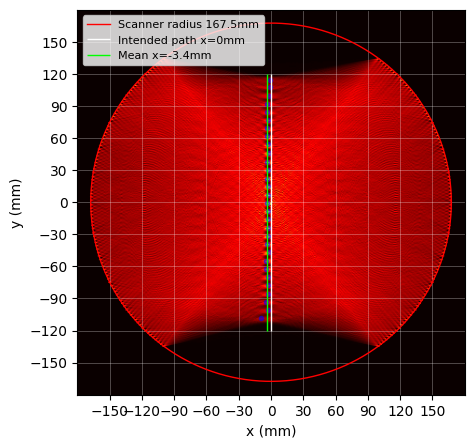
\includegraphics[width=0.5\textwidth]{images/vertpath.png}
    \caption{Siddon projection for vertical line source path at 30 1-second windows. Some offset from intended path.}
    \label{fig:vertpath}
\end{figure}

For our gaussian fitting, we actually observe two timing populations per module, which repeat in pattern across all modules. To account for this, we adopt a bimodal gaussian fit and take the update as the simple average of the two population means.

\subsection{Quantitative Validation}
We can look at the global time difference distribution (corrected for geometry) to see that time alignment correctly moves the distribution to 0 and tightens the width onto the CTR. Figure \ref{fig:ctr} shows the global time difference distribution for iterations 0, 1, 3, and 10. Figure \ref{fig:global4peaks} shows the 4 timing populations observed in the global distribution (as result of each module's 2 timing populations) converging onto each other at 0ps. 

Another analysis that is now possible is an estimate of the ``best'' CTR for the scanner by taking only coincidence events connecting the best performing left and right channels. Figure \ref{fig:bestctr} shows a heatmap of the timing FWHMs of all channels, and a CTR estimate computed only involving these best performing channels.







\begin{figure}[H]
    \centering
    \begin{tabular}{cc}
        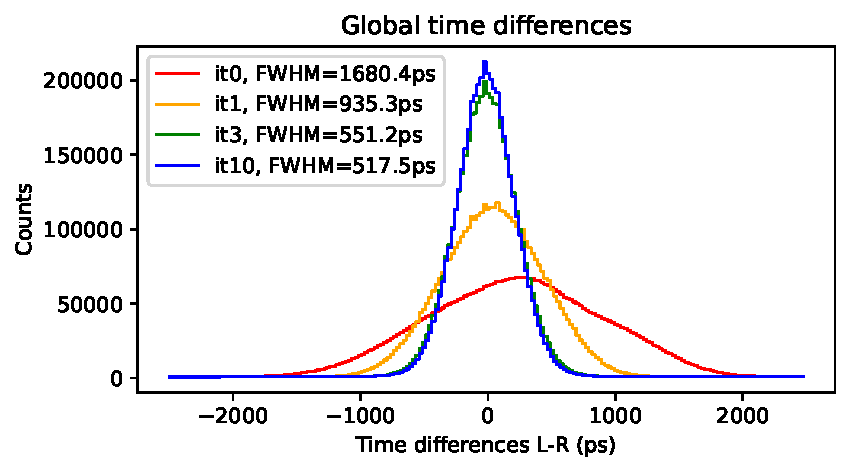
\includegraphics[width=0.45\textwidth]{plots/globalctr/globalctrhist.pdf} &
        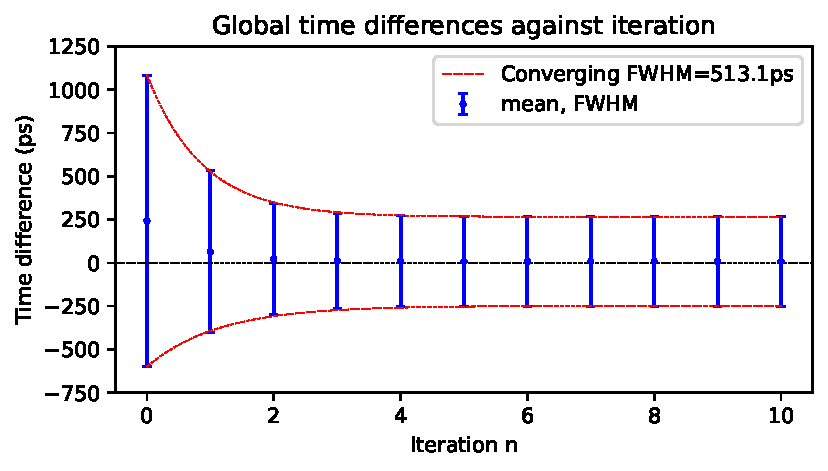
\includegraphics[width=0.44\textwidth]{plots/globalctr/globalctrplot.pdf} \\
    \end{tabular}
    \caption{Left: global time difference distirbution for iterations 0, 1, 3, and 10. Right: mean and FWHM of global distribution plotted across iterations 0-10, a fit of the FWHM suggests a converging FWHM of 513ps. This agrees with a per-LOR CTR calculation of about 520ps, which directly computes the FWHM of all coincidence events in high activity LORs.}
    \label{fig:ctr}
\end{figure}
\begin{figure}[H]
    \centering
    \begin{tabular}{cc}
        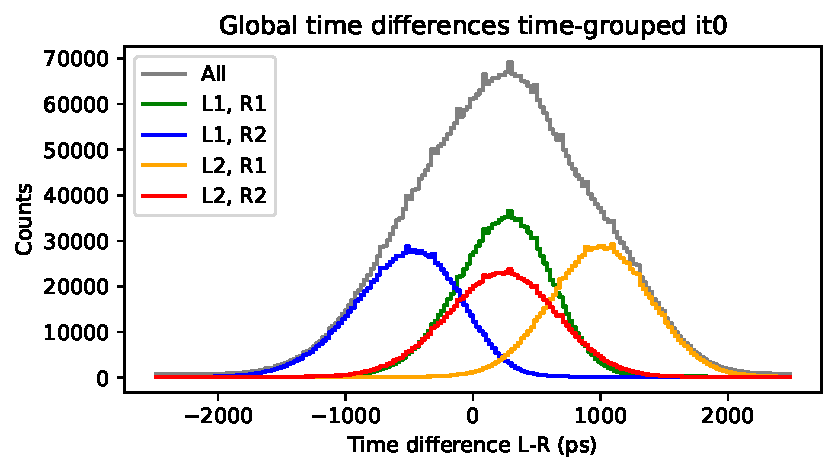
\includegraphics[width=0.44\textwidth]{plots/globalctr/fullscanner4peaksit0.pdf} &
        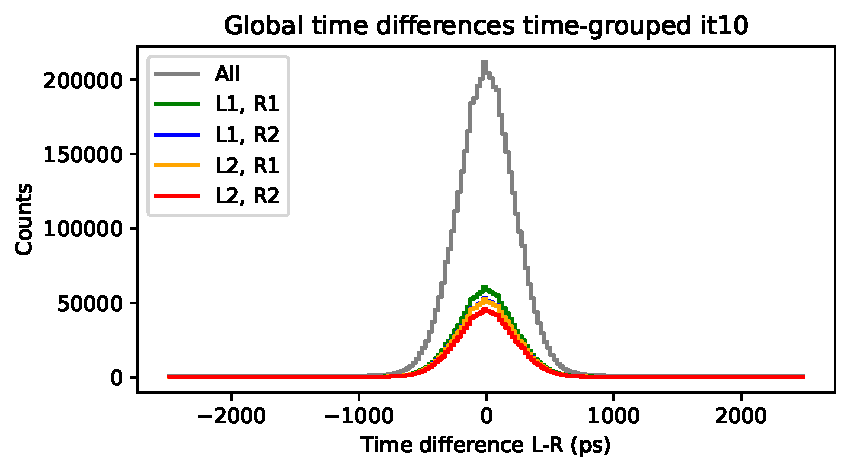
\includegraphics[width=0.45\textwidth]{plots/globalctr/fullscanner4peaksit10.pdf} \\
    \end{tabular}
    \caption{Left: global time difference distribution without calibration split into the 4 timing populations caused by each module's 2 populations, giving 4 combinations. Right: with calibration, the 4 populations converge onto each other at 0ps.}
    \label{fig:global4peaks}
\end{figure}
\begin{figure}[H]
    \centering
    \begin{tabular}{cc}
        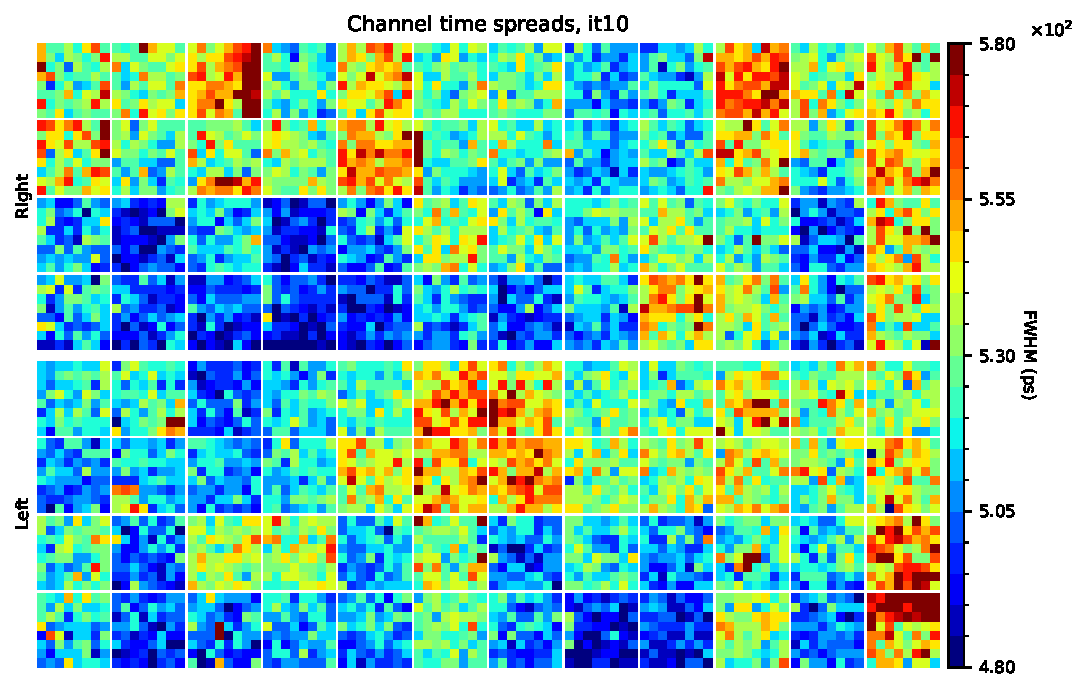
\includegraphics[width=0.45\textwidth]{plots/timecalconv/Channel time spreads, it10.pdf} &
        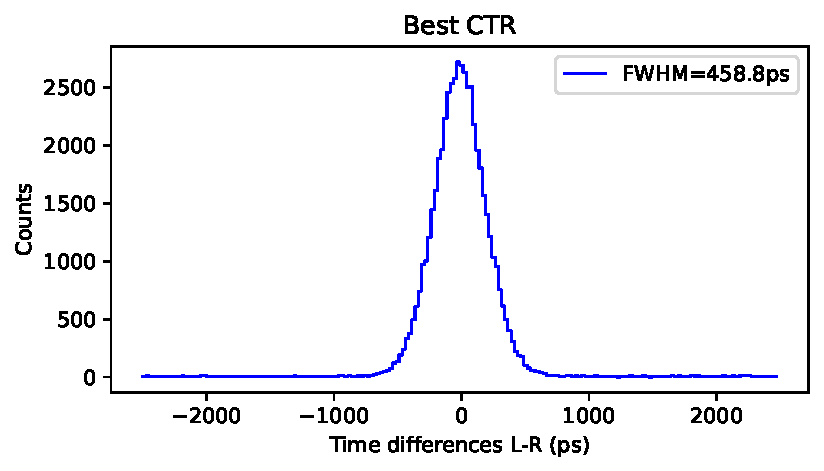
\includegraphics[width=0.44\textwidth]{plots/globalctr/bestctr.pdf} \\
    \end{tabular}
    \caption{Left: heatmap of the timing FWHMs of all channels. Right: CTR estimate computed only involving only 10\% best performing channels. We see improvement of roughly 11\% in the CTR estimate. }
    \label{fig:bestctr}
\end{figure}

\newpage
\section{Additional Comments}
Both normalization and time alignment follow a similar apprach to solve, with their forward models and iterative algorithms being nearly identical. The relation is made very explicit by taking the logarithm or exponentiation to transform between multiplicative and additive forward models. They also both follow the same general ideology for run design and methodology for computation of the target matrix. The only difference is the computation mechanism of the ratio or residual. 

\subsection{Uncertainty Treatment}
Both algorithms iterate against $g$, which is considered to be ``certain''. However there is some systematic error in $g$ due to the source shape, and there is also  Poisson statistical variation in $g$ due to the large number of channels. Currently, I have not considered any rigorous uncertainty treatment.

\begin{thebibliography}{9}
\bibitem{componentbasednormalization}
R D Badawi and P K Marsden, ``Developments in component-based normalization for 3D PET
'', \url{https://doi.org/10.1088/0031-9155/44/2/020}

\bibitem{timingoffset}
Li A, Zhang X, Zhou X, Fang L, Hu J, Li B, Zhang B, Xie Q, Li F, Xiao P. ``Timing offset calibration for TOF PET using stationary line source scans at multiple positions.'' \url{https://doi.org/10.1088/1361-6560/ad6edb}

\bibitem{mlemalgorithm}
Jinyi Qi and Richard M Leahy. ``Iterative reconstruction techniques in emission computed tomography.'' \url{https://doi.org/10.1088/0031-9155/51/15/R01}

\bibitem{tof_mlem_jpet}
P. Moskal, D. Kamińska, et al. ``TOF MLEM Adaptation for the Total-Body J-PET with a Realistic Analytical System Response Matrix.'' \url{https://arxiv.org/html/2302.02967v3}

\bibitem{morozov_github}
TPPTsim \url{https://github.com/andrmor/TPPTsim}, \\TPPTbuilder \url{https://github.com/andrmor/TPPTbuilder}, and \\TPPTcoinc \url{https://github.com/andrmor/TPPTcoinc}, from Andrey Morozov's GitHub.

\bibitem{geant4}
Geant4.

\bibitem{castor}
CASToR.

\bibitem{tpptreferencemanual}
TPPT Reference Manual, John Cesar, on DocDB.

\end{thebibliography}



\newpage
\appendix{A}
\section{Note on Heatmaps}
The channel heatmaps used are ordered to match the correct ASIC module numbering in the scanner. The channel numbering then repeats on each ASIC.
\begin{figure}[h]
    \centering
    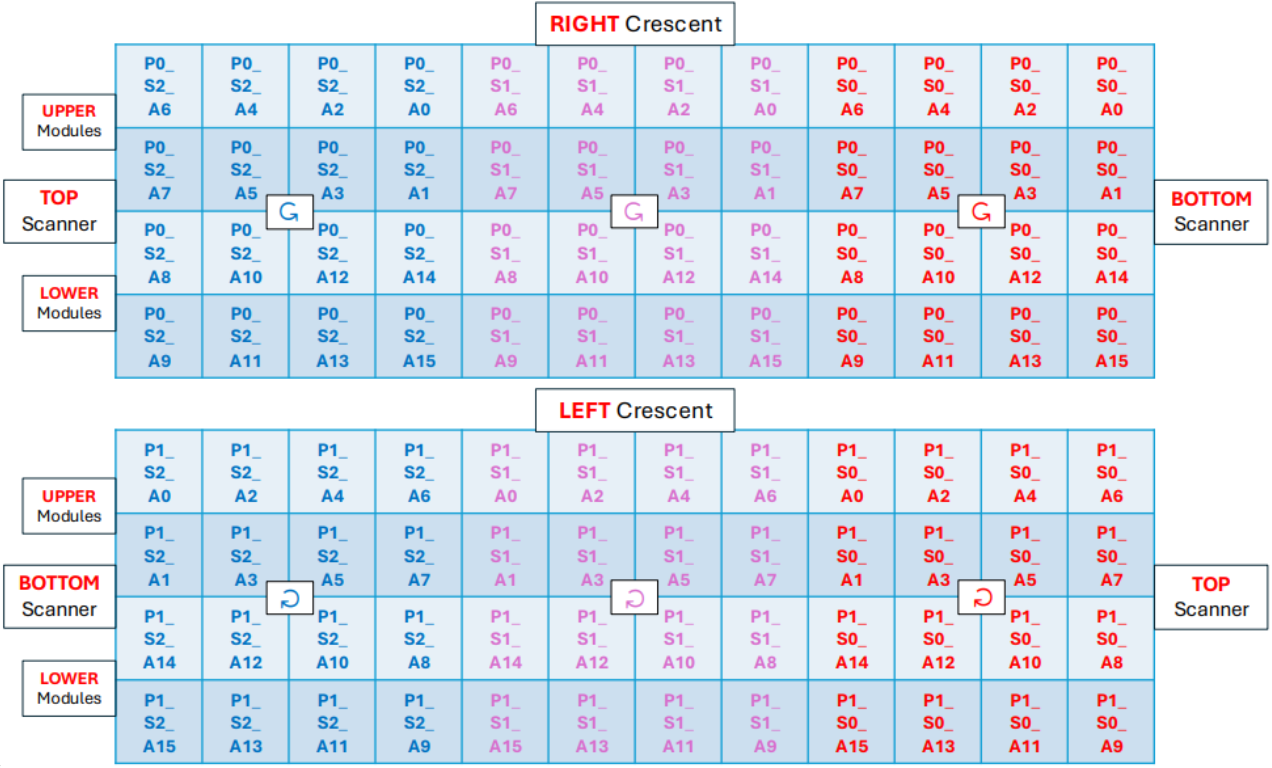
\includegraphics[width=0.75\textwidth]{images/channelmap.png}
    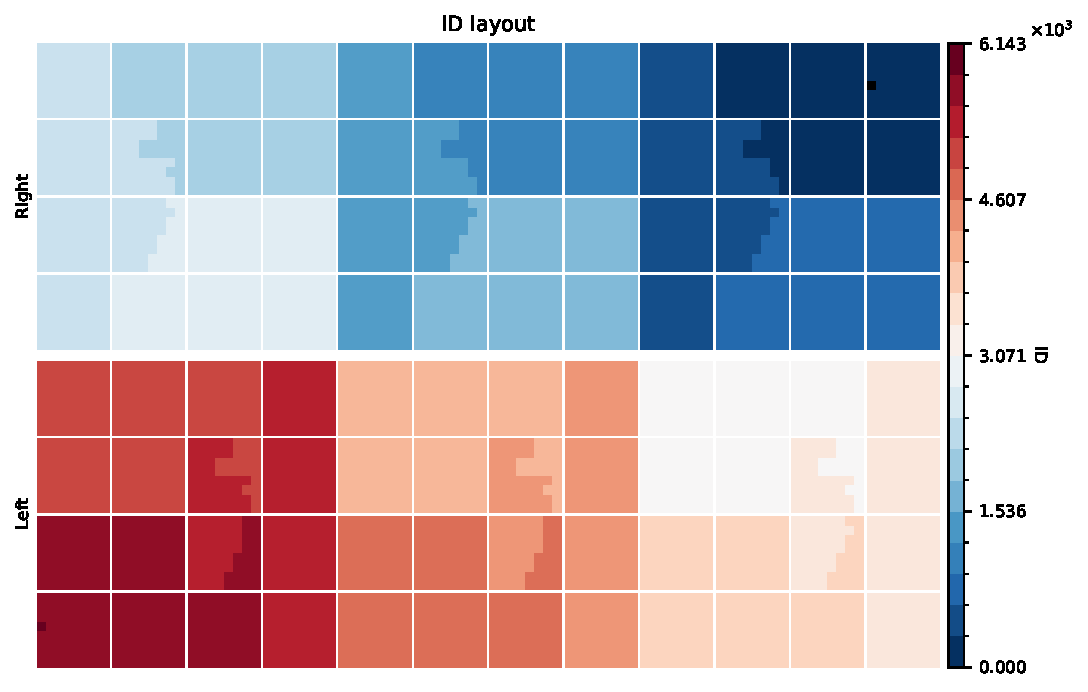
\includegraphics[width=0.75\textwidth]{images/ID layout.pdf}
    \caption{(top) Channel ASIC ID layout from [6]. (bottom) Heatmap ID layout. The channels are ordered to match the correct ASIC module numbering in the scanner. The channel numbering then repeats on each ASIC. I choose to use a discrete color scale for all heatmaps.}
    \label{fig:heatmap_order}
\end{figure}

\newpage
\section{Cuts Analysis}
The following are some inter-event time histograms used to check the behavior of data after these new geometric and duplicate cuts. ``Inter-event times'' (shortened intertime) are the time difference between consecutive events in the listmode data. Intertimes are binned for both left and right arcs, and should look essentially identical, an exponential from Poisson statistics (linear in log scale). The first histogram shows the intertimes after the photopeak cuts (the photopeak cuts are standard for us, will not be scrutinized here). The second histogram includes the geometric cuts, which over the entire data should just decrease the height of the distribution as events are removed without any time dependence. The third histogram includes the duplicate cuts, which should remove the peak at 0ps and paired events within the coincidence window, ideally leaving a flat distribution in the coincidence window region. We additionally see a small plateau at 100ns, which is the dead time, documented in PETsys ASIC data sheet. Typically this dead time is included as a multiplicative correction in normalization but for us it is so small it can be ignored.

\begin{figure}[H]
    \centering
    \begin{subfigure}{\textwidth}
        \centering
        \begin{tabular}{ccc}
            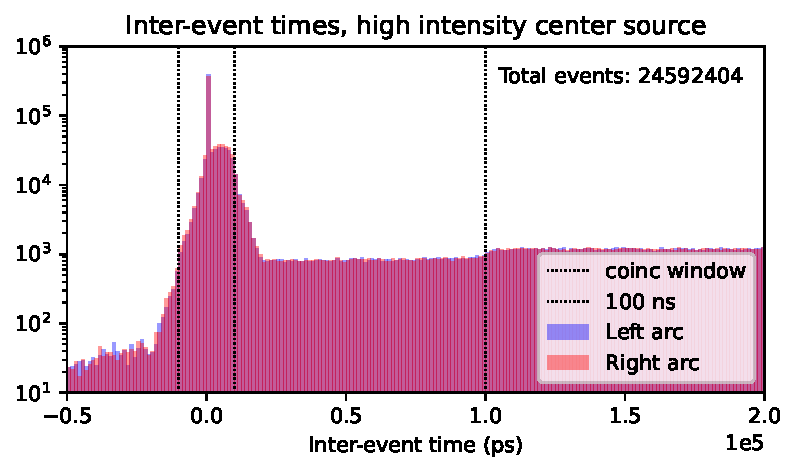
\includegraphics[width=0.3\textwidth]{plots/cutsanalysis/hcircpitimes.pdf} &
            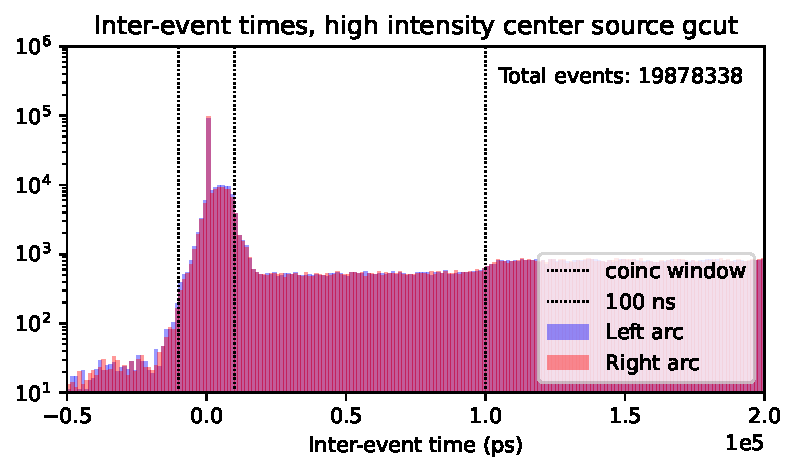
\includegraphics[width=0.3\textwidth]{plots/cutsanalysis/hcircpitimesg.pdf} &
            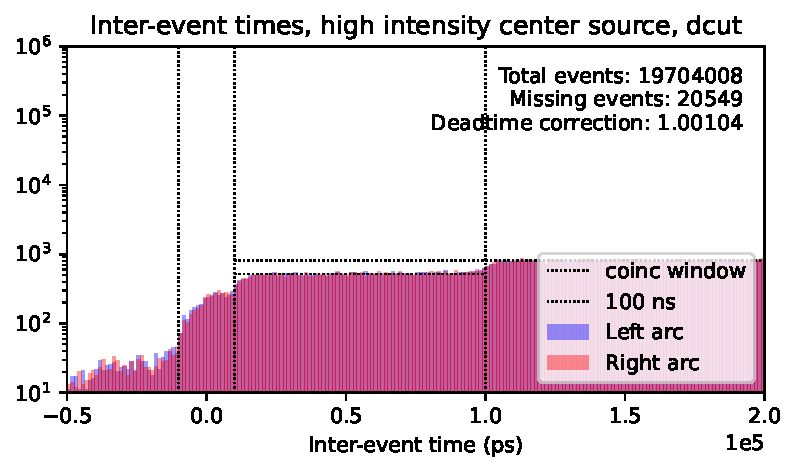
\includegraphics[width=0.3\textwidth]{plots/cutsanalysis/hcircpitimesgd.pdf} 
        \end{tabular}
        \caption{Circular scan source, left to right: with photopeak cuts only, photopeak cuts + geometric cuts, photopeak cuts + geometric cuts + duplicate cuts.}
        
    \end{subfigure}
    \begin{subfigure}{\textwidth}
        \centering
        \begin{tabular}{ccc}
            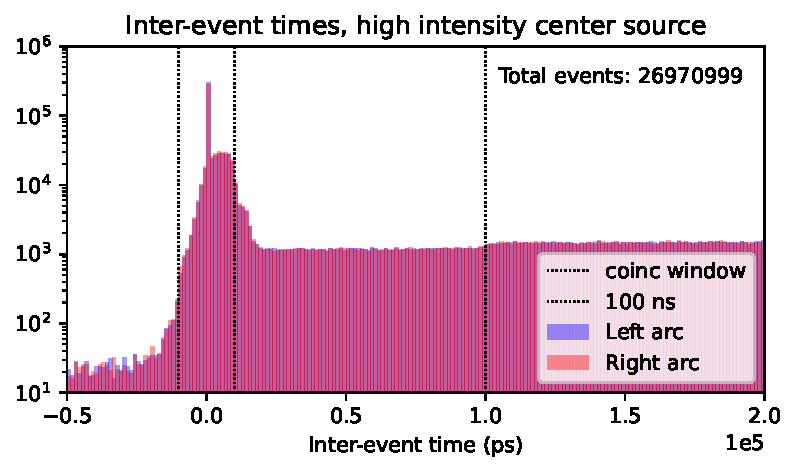
\includegraphics[width=0.3\textwidth]{plots/cutsanalysis/hvertpitimes.pdf} &
            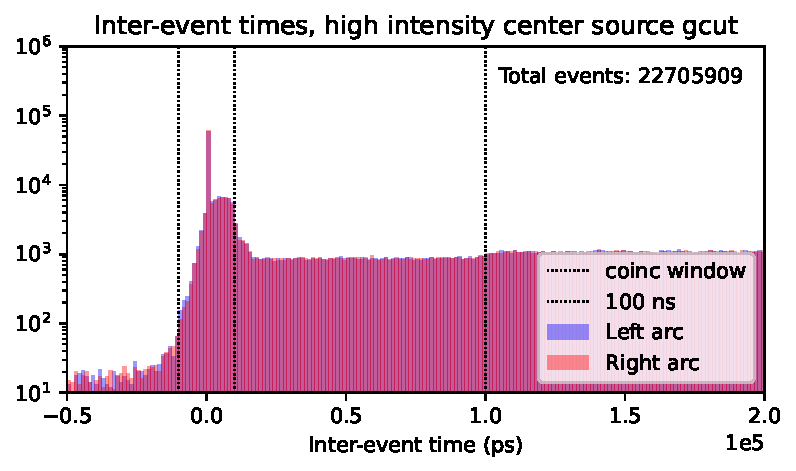
\includegraphics[width=0.3\textwidth]{plots/cutsanalysis/hvertpitimesg.pdf} &
            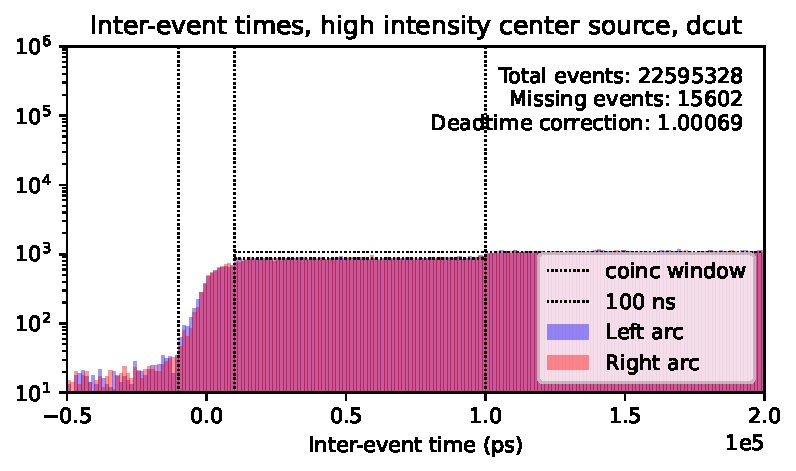
\includegraphics[width=0.3\textwidth]{plots/cutsanalysis/hvertpitimesgd.pdf}
        \end{tabular}
        \caption{Vertical scan source, left to right: with photopeak cuts only, photopeak cuts + geometric cuts, photopeak cuts + geometric cuts + duplicate cuts.}
    \end{subfigure}
    \caption{Inter-event time histograms used to check the behavior of data after these new geometrical and duplicate cuts.}
    \label{fig:cutsanalysis}
\end{figure}

\end{document}
